\NeedsTeXFormat{LaTeX2e}[2005/12/01]
%% scrbook - Ersatz für LaTeX book Klasse aus dem KOMA Script
%% Moegliche Optionen: diejenigen der Klasse scrbook ausser titlepage

%% deutsche Arbeit:
\documentclass[bachelor,       %% Typ der Arbeit: bachelor oder master
               twoside,        %% zweiseitiges Layout
               BCOR10mm,       %% Bindekorrektur 10 mm
%               liststotoc,nomtotoc,bibtotoc, %% Aufnahme der div. Verzeichnisse
                                              %% ins Inhaltsverzeichnis
               english,ngerman, %% Alternativspr. Englisch, Dokumentspr. Deutsch
%               ngerman,english  %% Alternativspr. Deutsch, Dokumentspr. Englisch
               final,          %% Endversion; draft fuer schnelles Kompilieren
%				draft,
               ]{GAUBM}

\usepackage{setspace}  %% Zur Setzung des Zeilenabstandes
\usepackage{babel}     %% Sprachen-Unterstuetzung
\usepackage{calc}      %% ermoeglicht Rechnen mit Laengen und Zaehlern
\usepackage[T1]{fontenc}       %% Unterstutzung von Umlauten etc.
%\usepackage[latin1]{inputenc}  %% 
%% in aktuellem Linux & MacOS X wird standardmaessig UTF8 kodiert!
\usepackage[utf8]{inputenc}    %% Wenn latin1 nicht geht ...

\usepackage{amsmath,amssymb} %% zusaetzliche Mathe-Symbole

\usepackage{lmodern} %% type1-taugliche CM-Schrift als Variante zur
                     %% "normalen" EC-Schrift
%% Paket fuer bibtex-Datenbanken
\usepackage{babelbib}
\selectbiblanguage{ngerman}
\bibliographystyle{apalikeGerman}

\newcommand{\tabheadfont}[1]{\textbf{#1}} %% Tabellenkopf in Fett
\usepackage{booktabs}                      %% Befehle fuer besseres Tabellenlayout
\usepackage{longtable}                     %% umbrechbare Tabellen
\usepackage{array}                         %% zusaetzliche Spaltenoptionen
\usepackage{siunitx}
\usepackage{verbatim}
% Mehrere Abbildungen nebeneinander
% Beispiel:
% \begin{figure}[htb]
%   \centering
%   \subfigure[<+Beschriftung 1+>\label{fig:<+label1+>}]
%   {\includegraphics[width=0.49\textwidth]{<+grafik1+>}}
%   \hfill
%   \subfigure[<+Beschriftung 2+>\label{fig:<+label2+>}]
%   {\includegraphics[width=0.49\textwidth]{<+grafik2+>}}
%   \caption{<+Beschriftung allgemein+>}
%   \label{fig:<+label-gesamt+>}
% \end{figure}
\usepackage{subfigure}

\usepackage{graphicx}
\graphicspath{{./Bilder/}}

\usepackage{adjustbox}
%Fußnoten zwingend auf diese Seite setzen
\interfootnotelinepenalty=1000

%keine Einrückung, wenn Latex doppelte Leerzeile
\parindent0pt

% Ableitungen: partiell: \pdv[n]{Q}{t} total \dv[n]{Q}{t} auch ohne [n] möglich
\usepackage{physics}

% Bra-Ket Vektor Notation für Quantenmechanik
\usepackage{braket}

% Für einheitsmatrix
\usepackage{bbm}

%Für mehrzeilige Gleichungen
%\usepackage{breqn}

\usepackage{xcolor}
\definecolor{elecgruen}{rgb}{0,0.66667,0}
%% umfangreiche Pakete fuer Symbole wie \micro, \ohm, \degree, \celsius etc.
\usepackage{textcomp,gensymb}

%\usepackage{SIunits} %% Korrektes Setzen von Einheiten
\usepackage{units}   %% Variante fuer Einheiten

%% Hyperlinks im Dokument; muss als eines der letzten Pakete geladen werden
\usepackage[pdfstartview=FitH,      % Oeffnen mit fit width
            breaklinks=true,        % Umbrueche in Links, nur bei pdflatex default
            bookmarksopen=true,     % aufgeklappte Bookmarks
            bookmarksnumbered=true  % Kapitelnummerierung in bookmarks
            ]{hyperref}

%% Weiter benoetigte Pakete: datenumber
%% Falls dieses Paket nicht in der Installation vorhanden ist,
%% kann es von der Seite mit diesem Template heruntergeladen werden
%% und in einem LaTeX bekanntem Verzeichnis installiert werden (notfalls
%% dem Verzeichnis mit der Arbeit).
\begin{document}
%%
%%                   Ab hier muessen die Anpassungen geschehen
%%
%% Hier den eigenen Namen einsetzen
\ThesisAuthor{Michael Alexander}{Lohmann}
%% Hier den Geburtsort einsetzen
\PlaceOfBirth{Randburg (RSA)}
%% Titel Arbeit. Das erste Argument ist der deutsche, das zweite der
%% englische Titel.
\ThesisTitle{Multi-Photon-Photoemission an Gold-Nanospitzen mit sichtbarem und nah-infrarotem Licht}{Multiphoton-photoemission at gold nanotips with visible and near-infrared light}
%% Erst- und Zweitgutacher/in
%% Ist der/die Betreuer/in nicht identisch mit dem/r Erstgutachter/in,
%% muss diese/r als optionales Argument angegeben werden.
\FirstReferee[Dr.\ Reiner Bormann und Benjamin Schröder]{Prof.\ Dr.\ Claus Ropers}
\Institute{4. Physikalischen Institut}
\SecondReferee{Prof.\ Dr.\ Christian Jooß}
%% Beginn und Ende des Anfertigungszeitraumes
\ThesisBegin{23}{5}{2016}
\ThesisEnd{29}{8}{2016}
%% DO NOT TOUCH THESE LINES!!!!
\frontmatter
\maketitle
\cleardoublepage
%% Zusammenfassung. Falls nicht gewuenscht, bitte auskommentieren.
\begin{abstract}
Ziel der Arbeit ist die erstmalige Untersuchtung des nichtlinearen Photoeffektes aus Gold-Nanospitzen über einen großen Wellenlängenbereich.
Dafür wurde ein Optisch Parametrischer Verstärker (OPA) verwendet, der Laserlicht mit kontinuierlich durchstimmbarer Wellenlänge liefert.
Der Laser-Puls wurde dazu verwendet, mit Multi-Photon-Photoemission Elektronen aus der Oberfläche auszulösen.\newline
Es zeigt sich, dass die Nichtlinearität (entspricht der Anzahl an benötigten Photonen) im untersuchten Bereich nicht stufenförmig (wie im einfachsten Modell), sondern annähernd linear ist.


%% Optional: Stichwoerter. Wenn nicht gewuenscht, koennen die beiden
%% folgenden Zeilen geloescht werden
  \bigskip\par
  \textbf{Stichwörter:} lokalisierte Elektronenemission, Gold Nano-Spitze, Multi-Photon Photoemission
\end{abstract}
%% So laesst sich in die andere Sprache umschalten (Englisch bzw. Deutsch)
\begin{otherlanguage}{english}
\begin{abstract}
The aim of this work is to determine the work function of Au nanotips.
An optic parametric amplifier was used to continuously vary the laser wavelength.
The fs-Laserpulses exracted electrons with multiphoton photoemission.\\
The results do show a nearly linear growth in the examined region instead of a stepfunction (like the simplest model).
  \bigskip\par
  \textbf{Keywords:} localized electron emission, gold nano-tip, multiphoton photoemission
\end{abstract}
\end{otherlanguage}

%% Ende des Vorspanns
\cleardoublepage
%% Ab hier 1 1/2 facher Zeilenabstand (durch setspace-Paket)
\onehalfspacing
%% Erzeugt Inhaltsverzeichnis
\tableofcontents

%% Hier kann man seine Bezeichnungsweisen erklaeren. Falls nicht
%% benoetigt, bis einschliesslich \end{nomenclature} auskommentieren
\begin{nomenclature}
%% Fuer die Berechnung der Spaltenbreiten muss \usepackage{calc}
%% geladen sein!
\section*{Lateinische Buchstaben}
\noindent
\begin{longtable}[l]{p{0.2\textwidth}p{0.7\textwidth-6\tabcolsep}p{0.1\textwidth}}
  \tabheadfont{Variable}&\tabheadfont{Bedeutung}&\tabheadfont{Einheit}\\\midrule\endhead
  $U_\text{Tip}$ & Spannung zwischen Spitze und Extraktor & $\unit{V}$\\
  $U_\text{Sup}$ & Spannung zwischen Suppressor und Extraktor & $\unit{V}$\\
  $U_p$ & Ponderomotive Energie & $\unit{J}$\\
  $e$ & Elementarladung & $\unit{Q}$\\
  $m_e$ & Elektronenmasse & $\unit{kg}$\\
  $I$ & Intensität des Lasers & $\unit{Wm^{-2}}$
\end{longtable}
\section*{Griechische Buchstaben}
\begin{longtable}[l]{p{0.2\textwidth}p{0.7\textwidth-6\tabcolsep}p{0.1\textwidth}}
  \tabheadfont{Variable}&\tabheadfont{Bedeutung}&\tabheadfont{Einheit}\\\midrule\endhead
  $\lambda$ & Wellenlänge & $\unit{nm}$\\
  $\omega$ & Frequenz & $\unit{Hz}$\\
  $\gamma$  & Keldysh-Parameter & $\unit{}$\\
  $\Phi$ & Austrittsarbeit & $\unit{eV}$
\end{longtable}
\section*{Indizes}
\begin{longtable}[l]{p{0.2\textwidth}p{0.8\textwidth-4\tabcolsep}}
  \tabheadfont{Index}&\tabheadfont{Bedeutung}\\\midrule\endhead
  $e$ & Elektron\\
  Tip & Nano-Spitze\\
  Sup & Supressor
\end{longtable}
\section*{Abk"urzungen}
\begin{longtable}[l]{p{0.2\textwidth}p{0.8\textwidth-4\tabcolsep}}
  \tabheadfont{Abkürzung}&\tabheadfont{Bedeutung}\\\midrule\endhead
  2D & zweidimensional\\
  3D & dreidimensional\\
  OPA & Optisch Parametrischer Verstärker\\
  MCP & Micro Channel Plate\\
  SHG & Second Harmonic Generation\\
  TEM & Transmissions Elektronen Mikroskop\\
  UTEM & Ultrafast TEM\\
  ULEED & Ultrafast Low Energy Elektron Defraction\\
  ATP & Above Threshhold Photoemission
\end{longtable}
\end{nomenclature}
%% \listoftables und \listoffigures sollten nur bei genuegender Anzahl Tabellen verwendet werden
%\listoffigures
%\listoftables

\mainmatter



\chapter{Einleitung}
Ein grundlegendes Verständnis der Materie ist ein essentielles Ziel der Forschung.
Daher wurden gerade seit den dreißiger Jahren des 19. Jahrhunderts immer ausgefeiltere Mikroskopietechniken entwickelt \cite{ruska_1931}.
Die höchsten räumlichen Auflösungen bieten hierbei noch immer Rastertunnelmikroskope (engl. \textit{scanning tunneling microscopy}, kurz STM) und Transmissionenelektronenmikroskope (\textit{transmission elektron microscope}, kurz TEM).
Deren Auflösungsvermögen, welches wichtig ist, um makroskopische Prozesse auch auf mikroskopischer Skala zu verstehen, liegt zwar auf atomarer Ebene ($\approx\SI{1}{\angstrom}$), jedoch ist die Zeitauflösung beider Methoden sehr begrenzt.
Gerade um dynamische Prozesse wie strukturelle Änderungen und Phasenübergänge zu untersuchen ist dies jedoch wichtig.
Um auch die temporale Auflösung zu erhalten, ist eine Elektronenquelle notwendig, welche räumlich kohärente kurze Elektronenpulse bereitstellt (z.B. \cite{gulde_ultrafast_2014}).

Eine Lösungsmöglichkeit besteht darin, Nanospitzen mit Femtosekunden-Laserpulsen zu beleuchten.
Die kleine Emissionsfläche, die durch Feldverstärkung und elektrostatische Felder auf den nanometrischen Apex begrenzbar ist, gewährleistet eine hohe räumliche Kohärenz der $e^-$-Pulse.
Dieser Ansatz wurde bisher schon erfolgreich in der ultraschnellen niedrigenergetischen Beugung von Elektronen (ULEED) und der ultraschnellen Transmissionselektronenmikroskopie (UTEM) verwendet (z.B. \cite{gulde_ultrafast_2014} und \cite{barwick_4d_2008}).
Dabei wird die hohe Zeitauflösung durch das Pump-Probe verfahren erreicht, bei dem das Experiment sehr häufig wiederholt wird und durch Aufnahmen zu unterschiedlichen Zeitpunkten ein Verlauf aufgenommen wird.
Ein Laserpuls regt beispielsweise einen Phasenübergang an.
Der Elektronenpuls trifft nun mit variabler Verzögerung auf die zu untersuchende Position und gibt ein variables Signal abhängig von dem momentanen Zustand der Probe zurück.
Dies ist allerdings nur machbar bei reversiblen Prozessen.

Um ein Elektron zu emittieren kann entweder die Energie eines einzelnen Photons ausreichen, um die Austrittsarbeit zu überwinden, oder es muss Multiphotonemission stattfinden.
Dabei treffen $N$ Photonen annähernd gleichzeitig auf ein Elektron.
Die Wahrscheinlichkeit der Emission ist proportional zu $I^N$, wobei $I$ die Intensität des einfallenden Lichtes beschreibt.

Allerdings stellten dabei zahlreiche Publikationen (s. Tab. \ref{tab:tip_andere_gruppen}) fest, dass bei der Intensität der emittierten Elektronen eine nicht erwartete Anzahl an benötigten Photonen benötigt wird.

In dieser Arbeit soll diese nichtlineare Photoemission einer systematischen Untersuchung über einen breiten Wellenlängenbereich erfolgen. Im genauen wird eine Gold-Nanospitze mit fs-Pulsen mit \SI{1.5}{\eV} bis \SI{2.7}{\eV} Photonenergie beleuchtet.

Um die Wellenlänge des Lasers verändern zu können wurde einen Optisch Parametrischen Verstärker (OPA) verwendet, mit dessen Hilfe sich die Wellenlänge des Lasers kontinuierlich von $250-\SI{20000}{\nano\meter}$ durchstimmen lässt.
Im Rahmen dieser Arbeit wurde der Bereich von 460 bis \SI{850}{\nm} untersucht.\newline\newline

Im Folgenden werden zunächst die Grundlagen der Arbeit erläutert, dann das Experiment erklärt und die Ergebnisse vorgestellt. Abschließend werden diese diskutiert.



\chapter{Grundlagen}
In diesem Kapitel werden die grundlegenden Begriffe und Formeln für diese Arbeit eingeführt, sowie die dahinterstehende Theorie erklärt.
Zunächst werden die Eigenschaften der Austrittsarbeit erklärt.
Dann wird ein Überblick über die verschiedenen Mechanismen der Photoemission gegeben, bevor die Multiphoton-Photoemission mit Hilfe der Störungsrechnung hergeleitet wird.
Die für diese Arbeit wichtigsten Aspekte werden mit der Fowler-DuBridge-Theorie erklärt.
Folgend wird der Schottky-Effekt erläutert, bevor abschließend eine kurze Bemerkung über die elektronische Zustandsdichte gemacht wird.


\section{Austrittsarbeit}
Mit dem Begriff Austrittsarbeit wird die Energie bezeichnet, die benötigt wird, um ein Elektron aus einem Atom oder Festkörper zu entfernen.
Sie ist material- und strukturspezifisch. 

Für das in dieser Arbeit verwendete Gold sind in Tabelle \ref{tab:austrittsarbeit} einige Messwerte aufgeführt, welche mit verschiedensten Methoden an ebenen Oberflächen ermittelt wurden.
Zu erkennen ist, dass sie von der jeweiligen Kristallfläche abhängt.
Aber auch bei der gleichen Kristallebene finden sich Unterschiede in den Ergebnissen (z.B. gibt es zu der (1 1 1)-Ebene Messwerte von 5.3 bis \SI{5.5}{\eV})


\begin{table}[h!]
\centering
\begin{tabular}{|l|c|c|c|}
\hline 
Quelle & Kristallfläche & Austrittsarbeit [\unit{eV}] & Methode \\ 
\hline\hline
\cite{fowler_1931} & ? 			& 4.9 				& th \\\hline
\cite{dubridge_further_1932} & ? 	& 4.81 			& ph \\\hline

\cite{sachtler_work_1966} & ? 	& \numrange{5.30}{5.45} & ph \\\hline

\cite{trasatti_operative_1974} & ? 	& 4.8 		& ec \\\hline
\cite{pescia_spin_1982} & (1 1 1) 	& 5.5 		& ph \\\hline
\cite{koetz_1986} & ? 				& $5.1\pm0.15$ 		& XPS \\\hline
\cite{lecoeur_1990}	& (1 1 1) 		& $5.30\pm0.05$ 	& ph \\
					& (3 1 1) 		& $5.16\pm0.07$ 	& Kontakt \\
					& (1 1 0) 		& $5.12\pm0.07$ 	& Kontakt \\
					& (2 1 0) 		& $4.96\pm0.07$ 	& Kontakt \\\hline
\cite{crc}		&(1 0 0) 			& 5.47 				& ph \\
 				&(1 1 0) 			& 5.37 				& ph \\
				&(1 1 1) 			& 5.31 				& ph \\\hline
\end{tabular} 
\caption{Auftragung verschiedener Austrittsarbeiten nach verschiedenen Publikationen. Abkürzungen Methoden: th $\equiv$ thermisch, ph $\equiv$ photoelektrisch, ec $\equiv$ elektrochemisch, XPS $\equiv$ Röntgen-Photoelektron-Spektroskopie, Kontakt $\equiv$ Kontaktpotential zu (1 1 1)-Facette}
\label{tab:austrittsarbeit}
\end{table}

Misst man jedoch nicht an glatten Oberflächen, sondern an Nano-Strukturen, so können noch weitere Effekte die Austrittsarbeit verändern (s. Kap. \ref{sec:erklaerung_lin}).
Desshalb sind auch die Daten interessant, welche andere Arbeitsgruppen mit ähnlichen Aufbauten, wie dem hier verwendeten ermittelten.
Einige davon sind in Tabelle \ref{tab:tip_andere_gruppen} dargestellt.
Zu erkennen ist, dass sich die Austrittsarbeit zum Teil stark von der einer planen Oberfläche unterscheidet.

\begin{table}[h]
	\centering
	\begin{tabular}{|l|l|r|r|r|r|r||r|}
\hline	Quelle 	& Mat- & Radius & Wellenl. & Pulsl. & $U_\text{ext}$ & Nichtlin. & Energie\\
& erial & [nm] & [nm] & [fs] & [V] & & ges. [eV]\\\hline\hline

	\cite{bormann_2010} & Au   & 20		 & 830 			&	 & 	& (4-)5 & 6-7.5 \\\hline
	\cite{park_2012} & & & 1-\SI{1.5}{\micro\m} & 30 & & & \\\hline
	\cite{wimmer_2014} & Au & 7 & 800 & 50 & & & \\\hline
	\cite{vogelsang_2015} & Au & & 1600 & 16 & & 7 & 5.4\\\hline
	\cite{benni_15} & Au & 22 & 800 & 10 & & 4.7 & 7.3\\\hline
	\cite{schenk_2010} & W & $50\pm10$ & 800 & 6.5 & 150 & $\approx 3$ & $\approx 5.7$\\\hline
				& & & & & 450 & 2 & 4.9\\
	\cite{barwick_2007} & W & $\approx 40$ & 810 & 30 & 300 & 3 & 6.1 \\
				& & & & & 50 & 4 & 6.7\\\hline
	\cite{bormann_ea_2015} & W & 25 & 400 & 50 & & & \\\hline
	\cite{hommelhoff_2006} & W & 80 & 800 & 8 & & & \\\hline
	\cite{dombi_2010} & Ag & 2.8 & 795 & 5 & & $4.1\pm 0.1$ & 6.1\\
	(SPP Einkopplung an & rauer & Oberfl.) & & & & &\\\hline
	\end{tabular}
	\caption{Messungen mit ähnlichen Aufbauten. Die gesamte Energie ist berechnet durch Photonenenergie, Nichtlinearität und Schottky-Effekt soweit die Parameter angegeben waren.}
	\label{tab:tip_andere_gruppen}
\end{table}



\section{Mechanismen der Photoemission}
Photoemission (PES) beschreibt die Auslösung von Elektronen aus Materie durch Bestrahlung mit Licht.
Dabei muss die absorbierte Energie die Austrittsarbeit übersteigen.

PES lässt sich in mindestens fünf Bereiche unterteilen, welche sich in der eingestrahlten Intensität $I$ unterscheiden:
\begin{itemize}
	\item\textit{Klassischer (linearer) Photoeffekt}
	Der klassische Photoeffekt nach \textsc{Einstein} \cite{einstein1905} besagt, dass Elektronen aus einem Festkörper nur dann ausgelöst werden, wenn ein einzelnes Photon genügend Energie $W_\text{Ph}$ besitzt, um die Auslösearbeit $\Phi$ zu leisten.
	In einem einfachen Bild ist diese bedingt durch die unterschiedliche Ladung von Atomkern und Elektron, weshalb sich diese anziehen und Energie aufgewendet werden muss, um sie zu trennen.
	Die Bilanzgleichung lautet dann
	\begin{align*}
	W_\text{El}=W_\text{Ph}-\Phi\quad .
	\end{align*}
	Es muss also gelten $W_\text{Ph}\geq\Phi$, damit die kinetische Energie des Elektrons $W_\text{EL}$ positiv ist.
	Eine größere Photonenenergie bewirkt eine höhere Überschussenergie.
	Kann man diese messen, so kann man Rückschlüsse auf die Austrittsarbeit schließen und mit der Photoelektron Spektroskopie eine Analyse der Inhaltsstoffe einer Probe machen.
	Für typische Metalle gilt $\Phi\approx4\ldots\SI7\electronvolt$ was einer Wellenlänge von höchstens \SI{300}{\nm} entspricht \cite{crc}.
	Höhere Intensitäten des eingestrahlten Lichts führen zu einem größerem Elektronenstrom, jedoch nur, wenn die Photonenenergie ausreichend groß ist.
	\item \textit{Multi-Photon-Emission}
	Nach Einstein ist nur die Photonenenergie ausschlaggebend für die Fähigkeit des Lichtes, Elektronen zu emittieren.
	Allerdings trifft dies nur für kleine Intensitäten zu, da im Rahmen einer störungstheoretischen Betrachtung des Emissionsprozesses (s. Abschnitt \ref{sec:stoerungsrechnung}) gezeigt werden kann, dass für große Intensitäten des eingestrahlten optischen Feldes die Wahrscheinlichkeit mit $I^N$ ansteigt, dass $N$ Photonen annähernd gleichzeitig auftreffen und wechselwirken.
	Dann steht die Summe der Einzelenergien zur Verfügung und die kinetische Energie der Elektronen berechnet sich aus der folgenden Formel:
	\begin{align*}
		W_\text{El}=N\cdot W_\text{Ph}-\Phi \qquad .
	\end{align*}
%	Im Experiment lässt sich $N$ durch die Variation der eingestrahlten Lichtintensität bei gleichzeitiger Messung des Elektronenstroms bestimmen.
	

	\item \textit{Optische Feldemission}
	Bei höheren Intensitäten wird das Atompotential durch das eingestrahlte elektrische Feld derart verformt, dass ein elektronischer Tunnelprozess stattfinden kann.
	
	\item \textit{Photo-assisted field-emission} Dabei tunnelt das Elektron analog zur optischen Feldemission heraus, wird jedoch vorher durch ein oder mehrere Photonen angeregt, was die Tunnelwahrscheinlichkeit erhöht.
	
	\item \textit{Above Threshhold Ionisation}
	Absorbiert ein Elektron mehr Photonen, als es zum Überwinden der Austrittsarbeit benötigen würde, so kann es deutlich höhere kinetische Energien besitzen, als anders ausgelöste.
	
\end{itemize}
Eine Abschätzung, ob Photoemission oder Feldemission der dominante Prozess ist, liefert der \textsc{Keldysh}-Parameter \cite{keldysh1965}.
Dieser berechnet sich durch
\begin{align}
	\gamma=\sqrt{\frac{\Phi}{2U_p}}\qquad .
	\label{eq:keldysh}
\end{align}

Ist $\gamma\ll 1$ ($F$ groß $\Rightarrow$ optisches Feld grö{\ss}er als atomares Potential), so wird die Emission bestimmt durch das Tunneln der Elektronen.
Für $\gamma\gg 1$ ($F$ klein $\Rightarrow$ atomares Potential überwiegt) werden die Atome durch Multi-Photon Prozesse ionisiert.\newline
Die in dieser Arbeit verwendeten Parameter führen zu $12\leq\gamma\leq22$.
Es ist also Multi-Photon-PES zu erwarten.

In der Formel wird mit $U_{p}$ die ponderomotive Energie bezeichnet, welche der mittleren kinetischen Energie der Elektronen im oszillierenden Lichtfeld entspricht:
\begin{align}
	U_p=\frac{e^2F^2}{4m_e\omega^2} \quad .
	\label{eq:ponderomotiv}
\end{align}
Hierbei bezeichnet $e$ die Elementarladung, $m_e$ die Elektronenmasse, sowie $F$ die elektrische Feldstärke an der Spitze, welche mit der Frequenz $\omega$ oszilliert.
Die kinetische Energie der Elektronen ist nach dem Auslösen nicht konstant, da das elektrische Feld sich verändert (zeitlich und räumlich) und so das Elektron immer wieder beschleunigt und verzögert wird.

Die elektrische Feldstärke wird durch die Feldverstärkung an Nanostrukturen verstärkt.
Dies bedeutet, dass die Feldlinien, welche senkrecht auf der Oberfläche stehen, bei kleinen Krümmungsradien dichter beieinander liegen, was einem stärkerem Feld entspricht (s. \textit{Lightning-Rod-Effect}).
Für eine Kugel mit Radius $r$, an der eine Spannung $U$ anliegt, ist das elektrische Feld $E=\frac{U}{r}$ (Gaußsches Gesetz für eine Kugel und $\vec E=-\nabla U$).
Die sogenannte Feldverstärkung ist das Verhältnis von verstärktem zu eingestrahltem Feld.
Für die hier verwendete Spitze beträgt sie nach \cite{benni_15} für den beleuchteten Apex $3.8$ .
Dies ist nach \cite{thomas_2016} ein häufig zu findender Wert, auch wenn es für Goldspitzen auch viele andere Messungen gab (z.B. \cite{ropers_2007} mit einem Wert von 10).\newline\newline

Im folgenden wird die Theorie der Multiphoton-PES mit Hilfe einer störungstheoretischen Herleitung erklärt.

\section{Störungstheoretische Herleitung}
\label{sec:stoerungsrechnung}
Die im letzten Kapitel beschriebene Multi-Photon-Emission lässt sich anhand einer störungstheoretischen Betrachtung herleiten.
Die Herleitung erfolgt dabei analog zu der Literatur von \cite[S. 29ff]{faisal} und \cite{laplance_1976}.
Dabei wird das Atompotential $H_0$ durch das zeitabhängige Potential des elektrischen Feldes erweitert, wodurch die zeitabhängige Schrödingergleichung für die Wellenfunktion $\psi$
\begin{align}
	i\hbar\pdv{}{t}\Psi(t)=[H_0+ V(t)]\Psi(t)
	\label{eq:schroedinger}
\end{align}
lautet.
Geht $V(t)\rightarrow0$ für $t\rightarrow\pm\infty$, so kann man mit
\begin{align*}
	\Psi(t)=\exp\left( -iH_0t/\hbar \right)\psi(t)
\end{align*}
Gleichung \ref{eq:schroedinger} durch
\begin{align}
	i\hbar\pdv{}{t}\psi(t)=\hat V(t)\psi(t)	
	\label{eq:schroedinger_kompakt}
\end{align}
ersetzen.
Dabei ist das neue Interaktionspotential $$\hat V(t)=\exp\left( iH_0t/\hbar \right)V(t)\exp\left( -iH_0t/\hbar \right)$$ (i.A. zeitabhängig, auch wenn $V(t)$ zeitunabhängig ist).

Die Energie-Eigenzustände $\ket i$ des ungestörten Atompotentials genügen $$H_0\ket i=\hbar\omega_i\ket i$$
und werden als bekannt vorausgesetzt.
Eine Lösung für Gleigung \ref{eq:schroedinger_kompakt} ist
\begin{align}
	\ket{\psi_i}=\ket i+\left( -i/\hbar \right)\int\limits_{-\infty}^tV(t')\ket{\psi_i(t')}dt'	\label{eq:psi_i}
\end{align}
wenn das Elektron ursprünglich im Zustand $\ket i$ war (für $t\rightarrow-\infty$ offensichtlich erfüllt).
Leitet man $\psi_i$ nach der Zeit ab, so ist Formel \ref{eq:schroedinger_kompakt} offensichtlich erfüllt.

Ist der Endzustand $\ket f$, so ist die Übergangswahrscheinlichkeit von $\ket i$ nach $\ket f$ natürlich $\left|\braket{f|\psi_i(t)}\right|^2$.
Der Zustand $\ket{\psi_i(t)}$ kann auch als
\begin{align}
	\ket{\psi_i(t)}=A(t)\ket i \label{eq:psiA}
\end{align}
geschrieben werden, wobei $A(t)$ der Amplitudenoperator ist.
Setzt man dies in Gleichung \ref{eq:psi_i} ein, so erhält man
\begin{align*}
	A(t)=\mathbbm{1}+\left( -i/\hbar \right)\int\limits_{-\infty}^tV(t')A(t')dt'
\end{align*}
oder durch Interiertes einsetzen
\begin{align}
	A(t)=\mathbbm1+\sum\limits_{N=1}^\infty A_N(t)
	\label{eq:A}
\end{align}
mit
\begin{align*}
	A_1(t)&=-i/\hbar\int\limits_{-\infty}^tV(t_1)A(t_1)dt_1\\
	A_N(t)&=(-i/\hbar)^N\int\limits_{-\infty}^tV(t_1)\int\limits_{-\infty}^{t_1}V(t_2)\cdots\int\limits_{-\infty}^{t_{N-1}}V(t_{N})dt_N\cdots dt_2dt_1\qquad.
\end{align*}
Dabei bezeichnet $N$ die jeweilige Ordnung der Störungsrechnung.
Nimmt man eine Dipol-Wechselwirkung an, so lautet das Potential
\begin{align*}
	\hat V(t)=\exp\left( iH_0t/\hbar \right)\left[\mathbf E(t)\cdot\mathbf D\right]\exp\left( -iH_0t/\hbar \right)\qquad.
\end{align*}
mit dem elektrischen Feld $\mathbf E(t)=\frac{\mathbf E}{2}e^{i\omega t}+\frac{\mathbf E^*}2e^{-i\omega t}$, dessen maximale Amplitude $E$ ist, sowie dem Dipoloperator $\mathbf D$ des Atoms, für den definiert ist $D_\lambda:=\boldsymbol\varepsilon_\lambda\cdot\mathbf D$, wobei $\boldsymbol\varepsilon_\lambda$ der Polarisationsvektor der $\lambda$-Mode ist.
Dann kann (mit dem Limes $t\rightarrow\infty$) 
\begin{align*}
	\bra fA_1(\infty)\ket i=-2\pi i/\hbar\left[ \delta (\omega_i-\omega_f-\omega)\frac{E}{2}\bra fD_\lambda\ket i+\delta (\omega_i-\omega_f+\omega) \frac{E^*}{2}\bra fD_\lambda\ket i\right]\\
\end{align*}
und
\begin{align*}
	\begin{split}
	\bra fA_2(\infty)\ket i=-2\pi i/\hbar^2\left\{ \delta(\omega_i-\omega_f+2\omega)\sum\limits_j\frac{E/2\bra fD_\lambda\ket jE/2\bra jD_\lambda\ket i}{\omega_i-\omega-\omega_j}\right. \\
	+\delta(\omega_i-\omega_f)\left[ \sum\limits_j\frac{E^*/2\bra fD_\lambda\ket j (E/2) \bra jD_\lambda\ket i}{\omega_i+\omega-\omega_j}\right. \\
	\left. +\sum\limits_j\frac{(E/2)\bra fD_\lambda\ket j(E^*/2)\bra jD_\lambda\ket i}{\omega_i-\omega-\omega_j} \right]\\
	\left. +\delta(\omega_i-\omega_f-2\omega)\sum\limits_j\frac{(E^*/2)\bra fD_\lambda\ket j(E^*/2)\bra jD_\lambda\ket i}{\omega_i-\omega-\omega_j} \right\}
\end{split}
\end{align*}
berechnen.
Die $\delta$-Funktionen resultieren in der Energie-Erhaltung.
Zu bemerken ist, dass der $A_1$-Term bei der Berechnung der Übergangswahrscheinlichkeit mit $E^2\propto I$ skaliert (zu Bedenken ist das Betragsquadrat, was in den obigen Gleichungen noch nicht angewendet wurde).
Dies entspricht dem klassischen Einsteinschen Photoeffekt.
Der Störungsterm zweiter Ordnung ($A_2$-Term) ist dann wie zu erwarten proportional zu $E^4\propto I^2$ und entspricht einem zwei-Photonen-Prozess.
Für Terme höherer Ordnung lässt sich zeigen, dass die Übergangswahrscheinlichkeit der Therme $N$-ter Ordnung mit $I^N$ skaliert.

\newpage
\section{Fowler-DuBridge-Theorie der Multiphoton-Photoemission}
Die Multiphoton-PES kann durch die \textsc{Fowler-DuBridge}-Theorie beschrieben werden (s. \cite{bechtel_1977} und \cite{girardeau_1995}).
Nach ihr setzt sich der Elektronenstrom aus
\begin{align}
	J&=\sum_{N=0}^\infty J_N=\sum_N\sigma_NI^N \quad ,\label{eq:photostrom}
\end{align}
mit
\begin{align}
	\sigma_N=\alpha_NA\left(\frac{e}{\hbar\omega}\right)^N(1-R_\omega)^NT^2F\left(\frac{N\cdot \hbar\omega-\Phi}{k_BT}\right)\qquad&\text{(Wirkungsquerschnitt)}\label{eq:wirkungsquerschnitt}\\\nonumber\\
\text{und}\qquad F(x)=\int_0^\infty dy\ln \left(1+e^{-(y+x)}\right)\qquad &\text{(Fowler-Funktion).}\nonumber
\end{align}
zusammen.
Hierbei ist $A=\SI{120}{\A\cm^{-2}\K^{-2}}$ die Richardson-Konstante, $e$ die Elementarladung, $k_B$ die Boltzmann-Konstante und $R_\omega$ die Oberflächenreflektivität.
Des Weiteren ist $T$ die Temperatur, $\hbar\omega$ die Photonenenergie und $\alpha_N$ ist eine materialspezifische Konstante, welche die restlichen bisher unberücksichtigten Prozesse berücksichtigt (z.B. Streuung im Metall und Reflektionswahrscheinlichkeit an der Oberfläche) \cite{brogle}.
Mit der Fowler-Funktion wird die dominante Ordnung des nichtlinearen Prozesses ausgewählt.

Der Wirkungsquerschnitt ist somit ein Maß für die Wahrscheinlichkeit der $N$-Photonen-Emission.\\

Wichtig für diese Arbeit ist die Proportionalität des Elektronenstroms zu der Laserintensität mit der Potenz $N$, sowie die Tatsache, dass $\sigma_N$ für $N\leq\frac{\Phi}{\hbar\omega}$ und $N\gg\frac{\Phi}{\hbar\omega}$ sehr klein ist.\\\\

In den Messungen wurde statt der Intensität die Leistung $P$ mit einem Powermeter gemessen.
Da jedoch die Intensität die eingestrahlte Leistung pro Fläche ist und sich diese durch die Reduzierung der Intensität bei konstanter Wellenlänge nicht ändert, gilt $I\propto P$.
In einem doppellogarithmischen Plot verursacht die Proportionalität einen Achsenabschnitt, aber keine Steigungsänderung.

Nimmt man an, dass nur eine wohldefinierte Austrittsarbeit zu leisten ist und dass die $\sigma_i\sigma_j\propto\delta_{ij}$ sind, so müsste sich bei der Auftragung von  Nichtlinearität gegen Wellenlänge eine Stufenfunktion ergeben.
Dies entspricht dem Fall, dass $N\cdot\hbar\omega\geq\phi$ sein muss oder anders formuliert:
\begin{align}
	N(\omega)=\left\lceil\frac{\phi}{\hbar\omega}\right\rceil
	\label{eq:nomega}
\end{align}
wobei mit $\lceil x\rceil$ die Aufrundungsfunktion bezeichnet wird.\\

Die Austrittsarbeit kann jedoch zum Beispiel durch den sogenannten Schottky Effekt verändert werden.

\section{Der Schottky-Effekt}
\label{sec:schottky}
Der sogenannte \textsc{Schottky}-Effekt ermöglicht die Verringerung der Austrittsarbeit durch das Anlegen einer Spannung $U$.
Dies wird in der schematischen Abbildung \ref{fig:schottky} dargestellt.
Dies ist möglich, da sich Elektron und die induzierte Sipegelladung durch ihr unterschiedliches Vorzeichen in der Ladung anziehen (siehe unverändertes Potential in schwarz mit $U=\SI0\V$).
Auf langen Distanzen nimmt die Reduktion des Potentials durch die attraktive Bildladung jedoch ab, sodass zum Emittieren ohne zusätzliches Feld noch die volle Austrittsarbeit $E_\infty-E_F$ geleistet werden muss.
Wirkt jedoch eine elektrische Feldstärke (in diesem Fall eine angelegte Spannung zwischen Spitze und Extraktor, eingezeichnet in rot), so wird das Potential im Vergleich zu dem gestrichelten Fall ohne Spiegelladung um
\begin{align}
	\Delta W&=\sqrt{\frac{e^3F}{4\pi\epsilon_0}}
	\label{eq:schottky_dW}\\
	\text{mit\qquad}F&=\frac{U}{k\cdot r}
\end{align}
erniedrigt und es ergibt sich $\phi_\text{eff}=\phi-\Delta W$.
Dabei wird mit $k$ der geometrischer Abschwächungsfaktor bezeichnet.
Dieser bezieht die Tatsache mit ein, dass Teile des Feldes im Vergleich zu einer Kugel durch den Schaft abgeschirmt werden.
In der Literatur wird meist $k\approx5$ angenommen (z.B. \cite{barwick_2007} oder \cite{hommelhoff_2006}).
Für die hier verwendeten Parameter Spitzenradius $r=\SI{45}{\nm}$ und angelegte Spannung $U_\text{Tip}=\SI{100}{\V}$ ergibt sich eine Feldstärke von  $F=\SI{0.44}{\V\per\nm}$.
Daher wird die Austrittsarbeit um $\Delta W=\SI{0.8}{\eV}$ gesenkt.



\begin{figure}[h!]
\centering
\adjustbox{width=0.5\linewidth}{\input{Schottky.pdf_tex}}
\caption{Schematische Darstellung des Schottky-Effektes. Eingezeichnet ist das ungestörte potential in schwarz, das externe Feld in rot, das resultierende Potential in blau und das Potential ohne den Schottky-Effekt mit externem Feld gestrichelt. Deutlich zu sehen ist, dass mit dem Effekt die Austrittsarbeit von $\Phi$ auf $\Phi_\text{eff}$ gesenkt wird.\label{fig:schottky}}
\end{figure}





 




\section{Die Elektronische Zustandsdichte}
\label{sec:zustandsdichte}

Elektronen mit Spin $\nicefrac{1}{2}$ müssen dem Pauli-Prinzip genügen, nach dem sich keine zwei Elektronen in dem selben Zustand befinden können.
Dies führt dazu, dass mit dem hinzufügen von weiteren Elektronen zu einem System immer energetisch höhere Zustände besetzt werden müssen.
Mit einem Band werden viele energetisch dicht beieinander liegende mögliche Zustände bezeichnet.
In einem Isolator sind alle Bänder entweder komplett gefüllt, oder leer, was dazu führt, dass kein Strom fließen kann.
Auch sind die Bänder im Gegensatz zu einem Halbleiter so weit entfernt, dass keine Elektronen aus einem gefüllten Valenzband (zum Beispiel durch thermische Fluktuation) in ein leeres Band (Leitungsband) kommt.
Ist dies der Fall, so können sowohl Elektron, als auch Loch zu einem Stromfluss beitragen.
Bei Metallen ist mindestens eines der Bänder nur teilweise gefüllt, wodurch ein Strom fließen kann.

Durch die Interaktion zwischen Kristallgitter mit dem periodischen Potential und den Elektronen ergibt sich die sogenannte elektronische Zustandsdichte.
Mit der elektronischen Zustandsdichte werden die Anzahl von stationären Elektronenzuständen in einem Energieintervall und Volumen bezeichnet.

In Abb. \ref{fig:gold_zustandsdichte} ist diese für Gold aufgeführt.
Zu sehen ist, dass es um eine Größenordnung mehr Elektronen gibt, die im $d$-Band $\SI2{\electronvolt}$ weniger Energie besitzen, als die Fermi-Energie.
Dies bedeutet, dass zur Ionisierung zwar ungefähr ein Photon mehr benötigt wird, es jedoch auch deutlich mehr Elektronen gibt.

Aufgrund der Tatsache, dass ein drei-Photonen-Prozess bei gleicher Intensität deutlich unwahrscheinlicher ist, als ein zwei-Photonen-Prozess, dieser Unterschied jedoch nicht so stark bei höheren Ordnungen ist, ist zu erwarten, dass je höher die Nichtlinearität ist, mehr Elektronen aus dem $d$-Band gelöst werden.

\begin{figure}[h!]
	\centering
	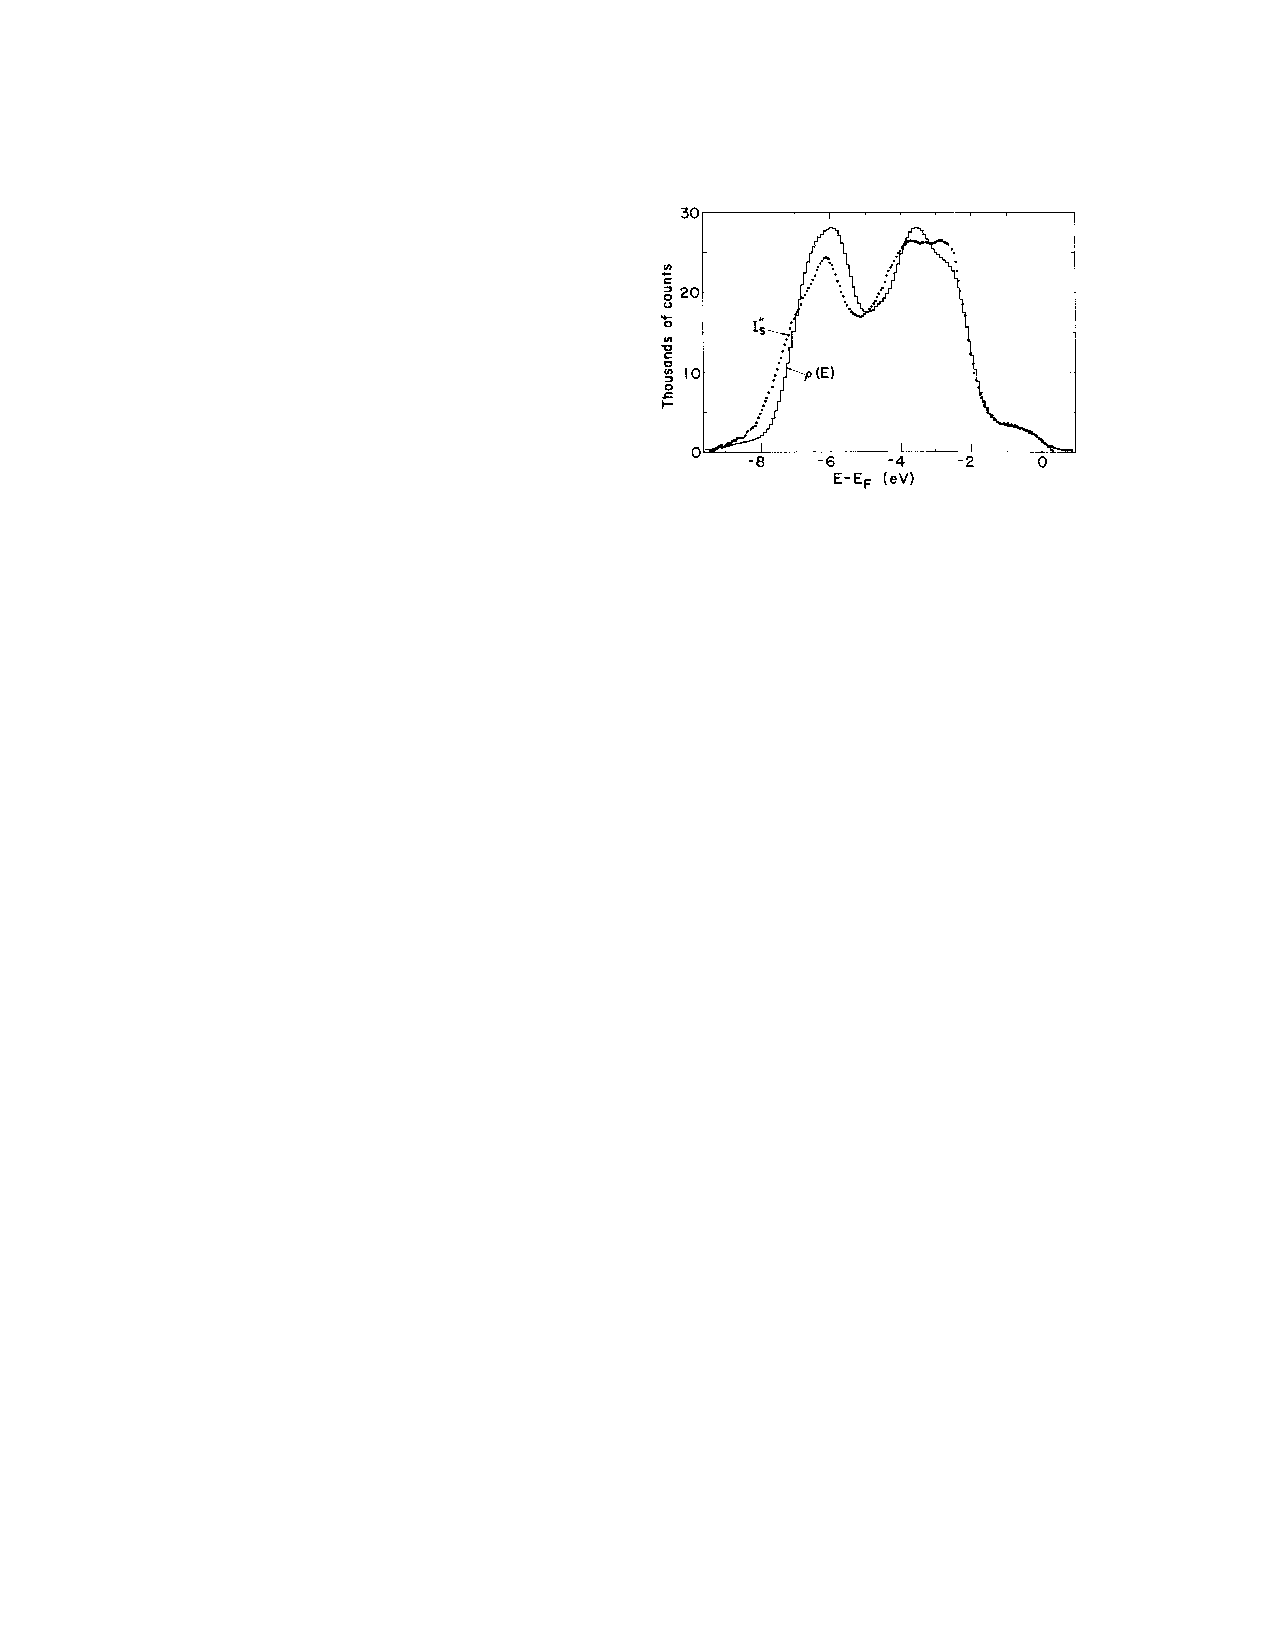
\includegraphics{GoldZustandsdichte}
	\caption{Elektronische Zustandsdichte aus \cite{gold_zustandsdichte}}
	\label{fig:gold_zustandsdichte}
\end{figure}


\chapter{Experimentelle Vorgehensweise}
Im Rahmen des folgenden Kapitels soll das verwendete Experiment näher erläutert werden.
Dazu werden Strahlengang, Kontrolle der Emission durch Supressor-Extraktor-Geometrie und Detektion erläutert.
Anschließend wird beschrieben, wie aus den Messdaten die Nichtlinearität ermittelt werden kann.\\


\section{Strahlengang}
In der hier vorgestellten Arbeit wurde der in Abb. \ref{fig:aufbau} dargestellte Aufbau verwendet.
Dieser beinhaltet einen fs-Laser (Details s. Kap. \ref{sec:laser}), dessen Leistung mit einem kontinuierlichen ND-Filterrad variabel abgeschwächt werden kann.
Der Laserstrahl ist in der Achse der Spitze polarisiert.
Um die Laserintensität zeitlich zu stabilisieren und zu steuern wird ein Teil des transmittierten Strahls mit einem Beamsplitter auf den Messkopf eines Powermeters geleitet, welches mit einer Feedback-Schleife das Filterrad steuert.
Der restliche Teil des Strahls wird mit einer in drei Richtungen beweglichen Linse auf die Spitze fokussiert.
Kleinere Fehler der Strahlposition werden so durch einen nicht zentralen Einfall auf die Linse korrigiert.


Die emittierten Elektronen werden (wie in Grafik \ref{fig:aufbau_kammer} dargestellt) zunächst mit der Beschleunigungsspannung $U_\text{Tip}$ zum Extraktor hin beschleunigt.
Der Supressor, dessen Spannung $U_\text{Sup}$ jedoch bei den hier durchgeführten Versuchen auf dem selben Potential (\SI{100}{\V}) lag, wie die Spitze, fokussiert den Elektronenstrahl, damit die Elektronen auf die MCP treffen.\newline

Anschließend treffen die einzelnen Elektronen (wie in Abb. \ref{fig:aufbau_kammer} zu sehen) auf eine Micro Channel Plate (MCP), welche ortsaufgelöst die Elektronen verstärkt.
Die austretenden Elektronenbündel treffen daraufhin auf einen Phosphorschirm, den sie punktuell zum Leuchten anregen.
Dieses kann nun mit einem CCD-Chip aufgenommen werden und dient als Datenquelle zur Auswertung.


\begin{figure}[h!]
	\centering
	\def\svgwidth{0.7\textwidth}
	\input{Aufbau3.pdf_tex}
	%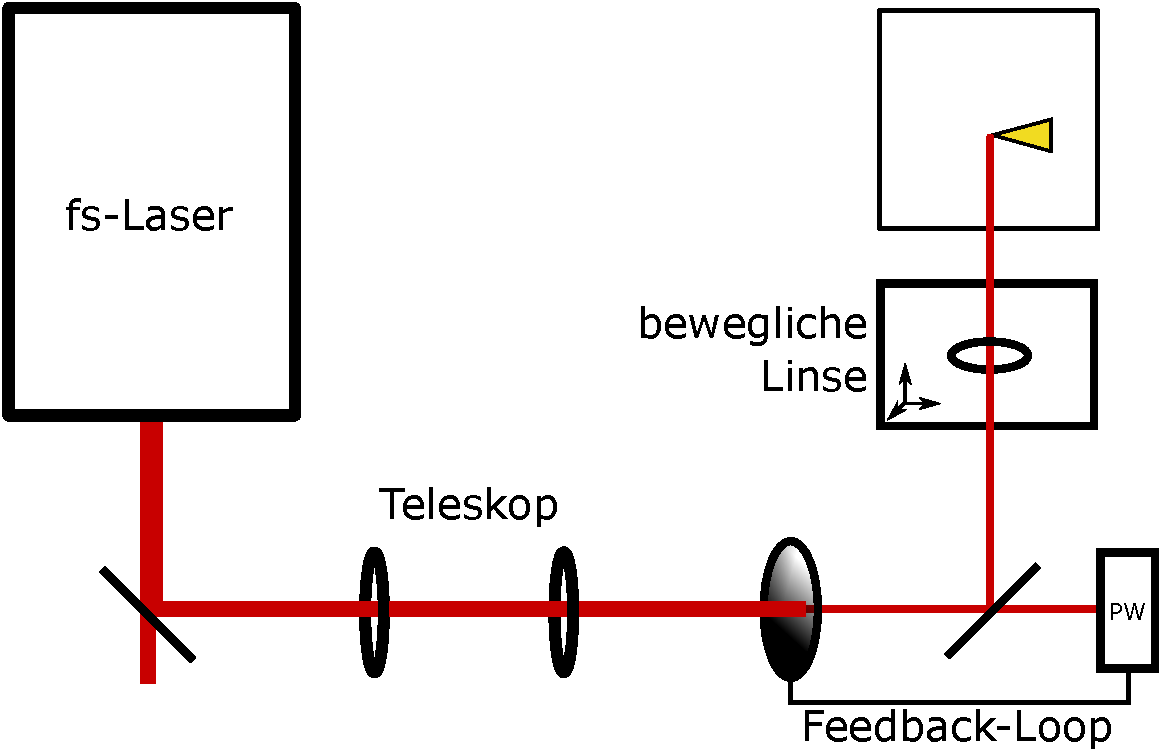
\includegraphics[width=0.8\linewidth]{Aufbau2}
	\caption{Schematischer Aufbau des Strahlengangs: Der Laserstrahl wird zunächst mit Hilfe eines Beamsplitters abgeschwächt, durch ein Teleskop (Vergrößerung 1:1)  kollimiert woraufhin die Laserleistung mit einem kontinuierlichen ND-Filterrad erneut reduziert wird. Dieses wird über einen weiteren Beamsplitter mit einem Powermeter (PW) in einer Feedback-Schleife gesteuert. Die Strahlposition auf der Spitze wird durch eine bewegliche Linse festgelegt.}
	\label{fig:aufbau}
\end{figure}

\subsection{Laser}
\label{sec:laser}
In dem verwendeten Aufbau wurde ein Lasersystem der Firma \textit{Light Conversion} verwendet.
Dieses besteht aus einem Pumplaser (\textsc{Pharos}), welcher \SI{200}{\fs} Pulse mit einigen $\unit{mJ}$ Pulsenergie und $\SI{100}{\kilo\hertz}$ Repetitionsrate zum Pumpen des Optisch Parametrischen Verstärkers (\textsc{Orpheus}) bereitstellt.
Dieser erzeugt wiederum Pulse mit Pulslängen von $\approx \SI{200}{\fs}$ in einem Resonator mit einem nichtlinearen optischen Kristall \cite{orpheus_tuningcurve}.
Dabei entstehen zwei Laserstrahlen unterschiedlicher Wellenlänge (das sogenannte Signal mit höherer Energie und Idler mit größerer Wellenlänge).
Um an dem Experiment nur einen der beiden zu bekommen, muss der andere mit einem Wellenlängenseparator getrennt werden.
Jedoch funktioniert die optisch parametrische Verstärkung nur in einem relativ kleinen spektralen Bereich um die eingestrahlten Frequenzen.
Wünscht man höhere Energien, so muss der Strahl mit Hilfe der Second-Harmonic-Generation (SHG) noch einmal frequenzverdoppelt werden.

Das Spektrum des Orpheus hat nach \cite{orpheus_tuningcurve} eine FWHM-Breite von $\SI5\nm$ bei einer Wellenlänge von \SI{700}{\nm} und von $\SI6\nm$ bei einer Wellenlänge von \SI{630}{\nm}.\\\\




\begin{comment}
<+rausnehmen+>$\Downarrow$
\section{Abhängigkeit der Anzahl an Elektronen von der Laser-Intensität am Gitter}
Zur Bestimmung der Abhängigkeit wurden von verschiedenen Wellenlängen von 460 bis \SI{850}{\nm} mit verschiedenen Belichtungszeiten (um eine Sättigung der Kamera bei zu hohen, aber auch eine zu geringe Anzahl an Elektronen bei kleinen Intensitäten zu vermeiden) und verschiedenen Laserintensitäten jeweils Bilder aufgenommen.
der Aufbau ist in Abb. \ref{fig:aufbau} zu sehen.
Dafür wurde zu Beginn noch mit einem manuellen Strahlabschwächer und Strahl blockieren durch den Powermeter-Messkopf, später automatisiert über eine motorisierte Bühne, welche über einen ständig durch einen Strahlteiler versorgten Messkopf gesteuert wurde, die Intensität des Lasers geändert.

Da zuvor während der Messungen jeweils ein zusätzlicher ND-Filter in den Strahlengang gestellt werden musste, weil das manuelle Rad nicht genügend abschwächen konnte, verschoben sich augenscheinlich einige Messwerte, so dass bei den manuellen Messungen die Kurven teilweise unverständliche Steigungen besaßen, welche auch nicht wiederholbar waren.
Ein weiterer wichtiger Grund für diese schwer zu interpretierenden Messungen war vermutlich, dass die MCP und der Kamera-Gain zu niedrig war, so dass der Algorithmus zum finden der Elektronen Probleme hatte, statistische Schwankungen von einem Signal zu trennen.
Dies sah man auch in den Bildern, bei denen der Algorithmus zunächst viele Schwankungen als Signal auffasste.
In Abb. \ref{fig:elektronen_bild} ist von beiden Messungen jeweils ein Bild exemplarisch dargestellt.

Da jedoch nicht alle Elektronen vom Gitter kamen, erwiesen sich einige Messungen jedoch als nicht sinnvoll, obwohl von dort deutlich mehr Elektronen kamen, als vom Apex.
Ich bekam jedoch augenscheinlich auch Elektronen vom Schaft oder vom Gitter selbst, da hier die Austrittsarbeit an der Kante vom 3 zu 4 Photonen bei $\SI{4.93}{\electronvolt}$, bei 2 zu 3 Photonen jedoch bei $\SI{4.6}\electronvolt$ lag.
Dies lag augenscheinlich daran, dass vom Gitter andere Elektronen ebenfalls aufgelöst werden konnten, welche nicht direkt vom Apex kamen.

\end{comment}
\section{Supressor-Extraktor Geometrie}
\begin{figure}[h!]
	\centering
	\def\svgwidth{0.8\textwidth}
	\input{Kammer_Aufbau_rot.pdf_tex}
%	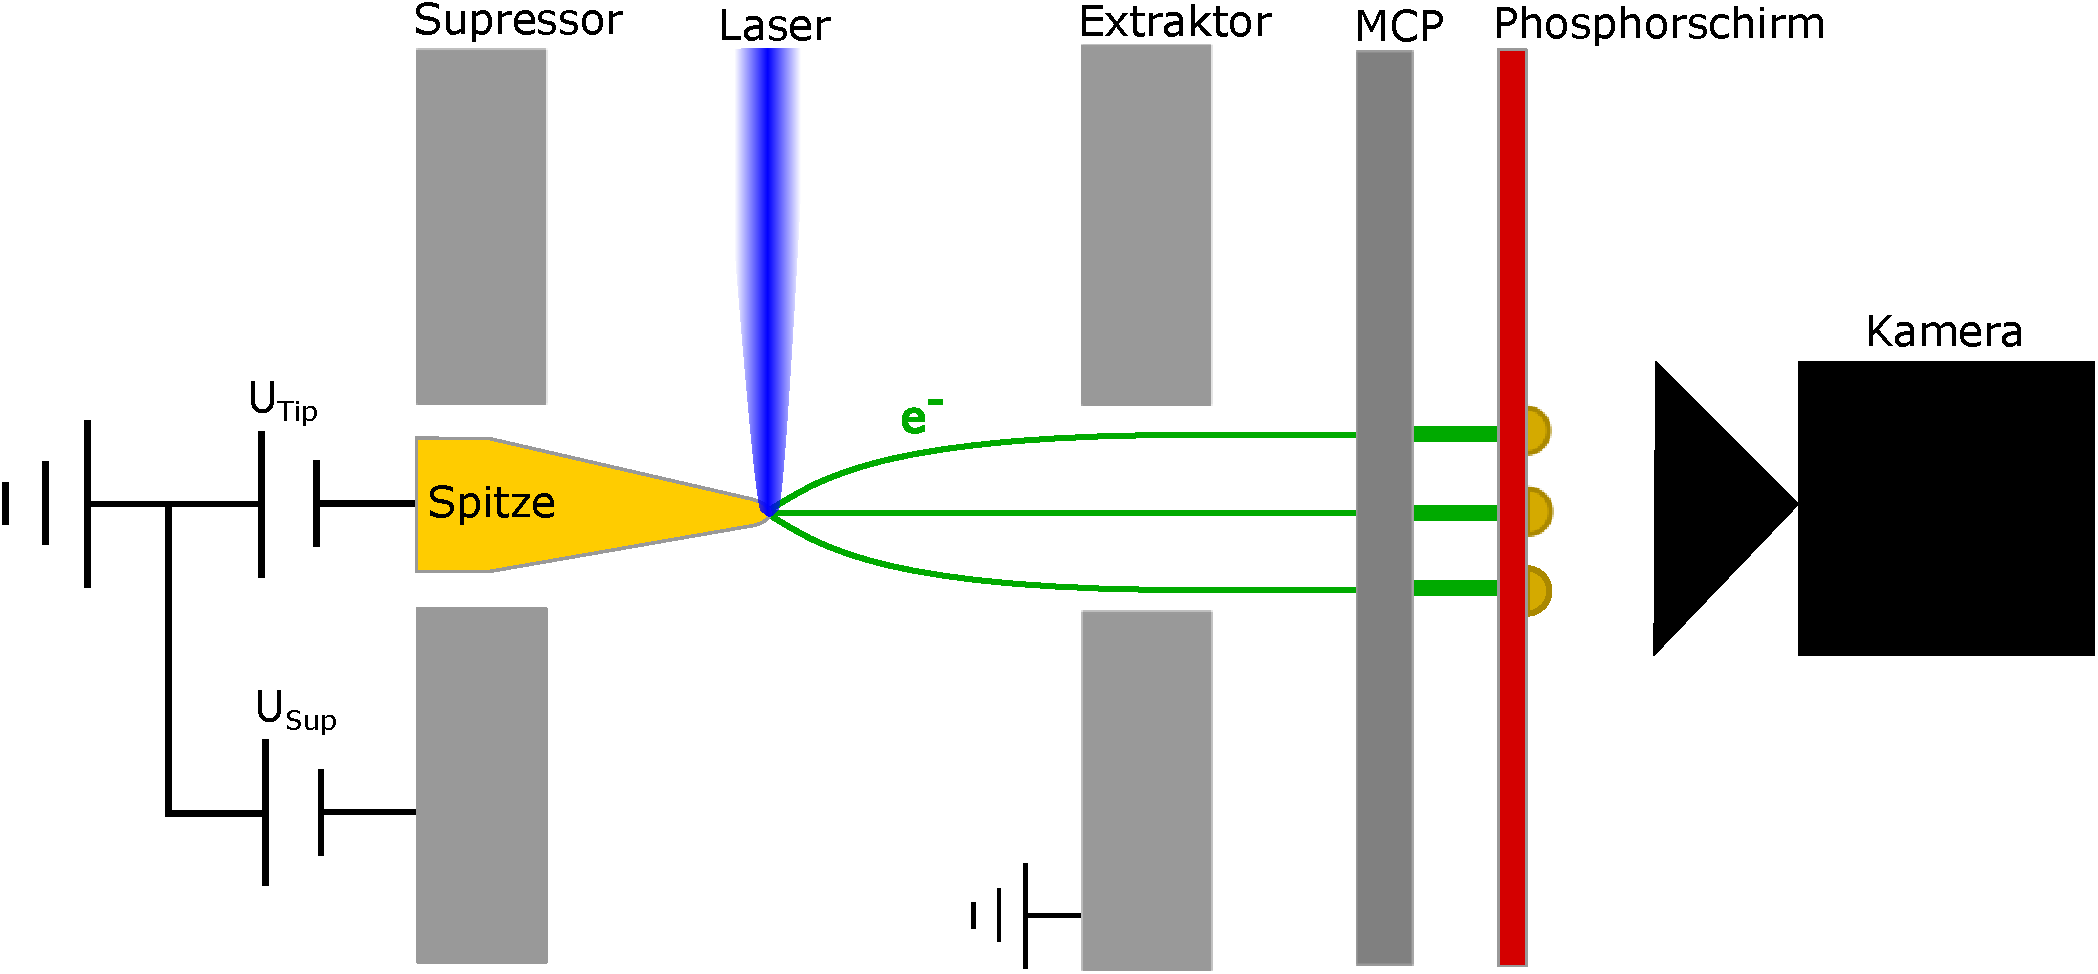
\includegraphics[width=0.9\textwidth]{Kammer_Aufbau}
	\caption{Detektion der Fotoelektronen: Die vom Laser aus der Spitze emittierten Elektronen werden durch die Spannung $U_\text{Tip}$ zum Extraktor hin beschleunigt. Durch $U_\text{Sup}$ kann der Emissionsort eingeschränkt und die Elektronen fokussiert werden. Mit Hilfe einer Micro Channel Plate (MCP) werden die Einzelelektronen verstärkt, so dass sie einen Phosphorschirm zum Leuchten anregen, was von einem CCD-Sensor aufgenommen wird.}
	\label{fig:aufbau_kammer}
\end{figure}
Die hier verwendete Geometrie (Abb. \ref{fig:aufbau_kammer}) besteht aus der Gold-Spitze, einem Supressor und einem Extraktor.

Die Spitze wurde aus einem geglühten Golddraht mit einem Durchmesser von \SI{0.25}{\mm} durch elektrochemisches Ätzen mit Salzsäure hergestellt (ausführliche Ausführungen hierzu in \cite{schmidt_2012} und \cite{neacsu_2007}).
Das anschlie{\ss}ende Ausglühen hat den Effekt, dass die zu Beginn polykristalline Struktur größere Körner gleicher Kristallstrukturen ausbildet.
Daher ist der Apex mit hoher Wahrscheinlichkeit monokristallin, was dazu führt, dass keine weiteren Facetten (und damit Austrittsarbeiten) durch Korngrenzen hinzukommen.

Die Abmaße des verwendeten Aufbaus sind in Abb. \ref{fig:aufbau_kammer} dargestellt.

%Zusätzlich besitzt die untersuchte Spitze ein mit dem Focused Ion Beam (FIB) eingraviertes Gitter, um Oberflächenplasmon-Polaritone (SPP) einkoppeln zu können.
%Um Apex und Gitter getrennt anregen zu können sind diese ca. \SI{45}{\micro\m} voneinander entfernt.
%Im Rahmen dieser Arbeit wurde sich jedoch darauf beschränkt, den Apex zu beleuchten, da das Gitter mit einer Periodizität von \SI{800}{\nm} nur in einem geringen Wellenlängenbereich eine effiziente Einkopplung der elektromagnetischen Wellen zulässt.
%Zusätzlich zu der nicht konstanten Einkopplung werden auch an dem Gitter Elektronen ausgelöst.

\section{Zählalgorithmus der Elektronen}
\label{sec:zaehlalgorithmus}
Für die Auswertung wurde der Elektronenstrom computergestützt ausgewertet.
Als Datenquelle dienten 2D-Intensitäts-Aufnahmen, welche von der Kamera aus Grafik \ref{fig:aufbau_kammer} aufgenommen werden.

Um die Anzahl der Elektronen auf den einzelnen Bildern zu bestimmen, gibt es zwei Möglichkeiten:
\begin{itemize}
\item Elektronen maschinell zählen: Ein Algorithmus, welcher in jedem Bild die Elektronen zählt.
	Von Vorteil ist, dass die Helligkeit der einzelnen Elektronen (sollte sie sich bei verschiedenen kinetischen Energien unterscheiden) keinen Einfluss auf die Detektion hat.
	Der Nachteil ist jedoch, dass möglicherweise falsche Elektronen detektiert werden oder vorhandenen (insbesondere bei hohen Intensitäten) nicht erkannt werden.
\item Helligkeit integrieren: Die Helligkeit der einzelnen Pixel über das ganze Bild summieren.
	Vorteilhaft an dieser Methode ist, dass gerade bei hohen Intensitäten der Algorithmus zuverlässiger ist.
	Sollten die Elektronen jedoch nicht vergleichbar in der Helligkeit sein (z.B. da die Kamera keine lineare Intensitätsskala besitzt),  gibt der Algorithmus eine falsche Anzahl heraus.
	Insbesondere kleine Anzahlen an Elektronen in einem Bild kann diese Methode nur schlecht ermitteln.
\end{itemize}

Da die verwendeten Bilder nur eine relativ geringe Anzahl an Elektronen besaßen, wurde das erste Programm zur Auswertung gewählt.
Dieses bestimmt zunächst aus Bildern ohne Elektronensignal die toten Pixel, indem er diejenigen aussortiert, welche über 100 Bilder gemittelt mehr als $120\%$ des Mittelwerts haben.
Dies wurde getan, um nicht versehentlich scheinbare Elektronen zu detektieren, welche aus fehlerhaften Pixeln des CCD-Chips resultieren können.

Im Folgenden werden die Elektronen in der Region Of Interest (ROI - dem Bereich des Bildes, der tatsächlich den Phosphorschirm beinhaltet) gezählt.
Damit das Rauschen einen möglichst geringen Effekt hat, werden alle Pixel unter einer bestimmten Schwelle (hier einem Wert von 12, da fast alle Pixel in einem unbeleuchteten Bild unter diesem Wert liegen) auf Null gesetzt.
Dann wird das Bild gefaltet mit einer Matrix
$$A=\begin{pmatrix}
\nicefrac{1}{9} & \nicefrac{1}{6} & \nicefrac{1}{4} & \nicefrac{1}{6} & \nicefrac{1}{9} \\ 
\nicefrac{1}{6} & \nicefrac{1}{3} & \nicefrac{1}{2} & \nicefrac{1}{3} & \nicefrac{1}{6} \\ 
\nicefrac{1}{4} & \nicefrac{1}{2} & 1 & \nicefrac{1}{2} & \nicefrac{1}{4} \\ 
\nicefrac{1}{6} & \nicefrac{1}{3} & \nicefrac{1}{2} & \nicefrac{1}{3} & \nicefrac{1}{6} \\ 
\nicefrac{1}{9} & \nicefrac{1}{6} & \nicefrac{1}{4} & \nicefrac{1}{6} & \nicefrac{1}{9}
\end{pmatrix}$$
um verbleibendes Rauschen zu filtern.
Ein Beispiel für ein gefaltetes Bild ist in Abb. \ref{fig:460nm_109muW_gefaltet} dargestellt.
Nach einem weiteren Threshhold, über den die gefalteten Daten kommen müssen um weiteres Rauschen zu minimieren, werden die Maxima in den Daten gesucht.
Da dicht beienander liegende Elektronen nur ein gemeinsames haben, kann dieser Algorithmus solche nicht auseinanderhalten.
Die Anzahl und Position der Maxima in den verarbeiteten Daten sollte dann mit denen der Elektronen übereinstimmen.

\begin{figure}[ht!]
  \centering
  \subfigure[Wellenlänge $\SI{460}{\nano\meter}$, Belichtungszeit $\SI{10}{\milli\second}$, Laserleistung $\SI{109}{\micro\watt}$\label{fig:460nm_109muW}]
  {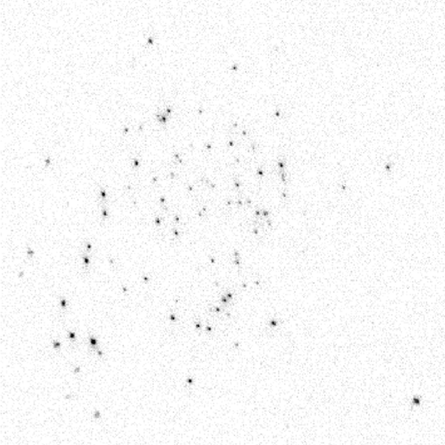
\includegraphics[width=0.45\textwidth]{460nm_109muW_10ms_g}}
    \hfill
  \subfigure[Bild (a) gefaltet mit Matrix $A$ \label{fig:460nm_109muW_gefaltet}]
  {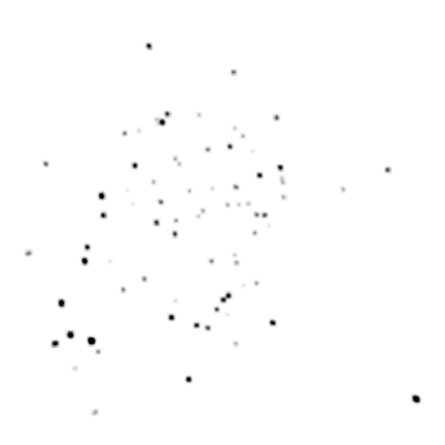
\includegraphics[width=0.45\textwidth]{460nm_109muW_10ms_gefaltet_g}}
  \hfill
  \subfigure[Bild (a) mit den vom Algorithmus gefundenen Elektronenpositionenin rot markiert. Die blau markierten scheinen auf den ersten Blick auch Elektronen zu sein, sind jedoch nur bis zu 4 Pixel im Durchmesser und daher vermutlich nur rauschen.\label{fig:460nm_109muW_e}]
  {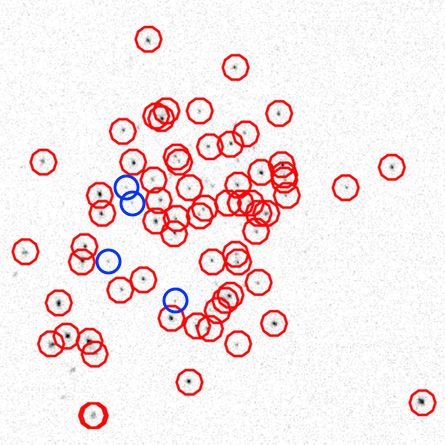
\includegraphics[width=0.45\textwidth]{460nm_109muW_10ms_e_g_fPos}}
%  \hfill
%  \subfigure[Wellenlänge $\SI{460}{\nano\meter}$, Belichtungszeit $\SI{10}{\milli\second}$, Laserleistung $\SI{308}{\micro\watt}$, Ausschnitt\label{fig:460nm_308muW}]
%  {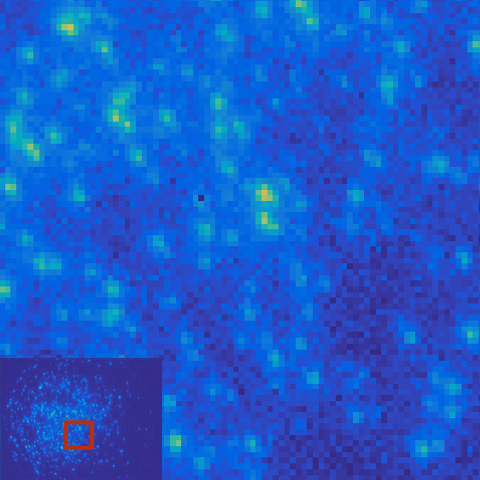
\includegraphics[width=0.49\textwidth]{460nm_308muW_10ms_ganz}}
%  \hfill
%  \subfigure[Bild links mit vom Algorithmus gefundenen Elektronenpositionen. Markiert sind in weiß Positionen mit vermutlich falsch detektierten Elektronen und in gelb nicht gefundene Positionen. Jedoch hat sich bei der betrachtung vieler Bilder herausgestellt, dass sich dies meist herausmittelt. \label{fig:460nm_308muW_e}]
%  {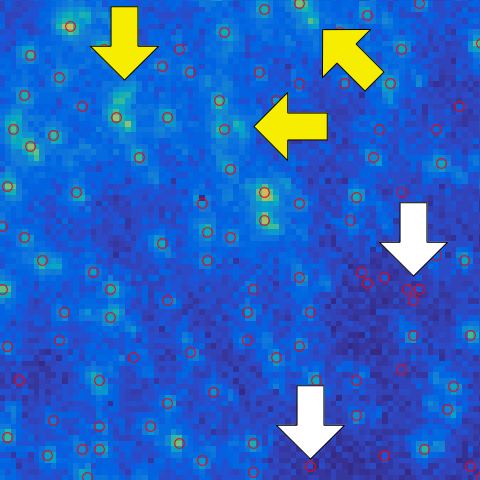
\includegraphics[width=0.49\textwidth]{460nm_308muW_10ms_e_p}}
  \caption{Vergleich von Aufnahmen des Phosphorschirms und den darauf gefundenen Elektronenpositionen}
  \label{fig:algorithmus}
\end{figure}
In Abb. \ref{fig:460nm_109muW} kann man die ROI eines typischen Bildes erkennen.
Zu erkennen ist, dass die Elektronen noch räumlich getrennt sind.
Daher ist es nicht verwunderlich, dass die in Bild \ref{fig:460nm_109muW_e} gefundenen Elektronen in guter Übereinstimmung mit den von Menschen erkannten liegen.
Einige Punkte, welche man auf dem Bild erkennt nicht detektiert wurden, liegt daran, dass die Farbskala sehr eingeschränkt ist und die Punkte nur sehr schwach sind.
Die blau umrandeten beispielsweise sind nur wenige Pixel im Durchmesser und können so auch durch Rauschen hervorgerufen worden sein und nur für das Auge dominant wirken.

Bei einer zu großen Elektronenanzahl (bzw. Belichtungszeit) kann der Algorithmus zwischen einzelnen Elektronen nicht mehr differenzieren.
Dies geschieht langsam und von der Mitte, wo die meisten Elektronen auftreffen, beginnend.
Daher sinkt in diesem Fall die Steigung der Messpunkte zum Beispiel in Diagramm \ref{fig:520e} langsam.





\section{Intensitätsabhängiger Photostrom}
Ein wesentliches Ziel der vorliegenden Arbeit ist die Bestimmung des intensitätsabhängigen Photostroms in Abhängigkeit der Wellenlänge.

Dabei wird der Photostrom in Abhängigkeit der Laserintensität bei konstanter Wellenlänge gemessen.
Nach Gleichung \ref{eq:photostrom} gilt $J\propto I^N$, wodurch sich $N$ als Geradensteigung in einem doppel-logarithmischen Plot ablesen lässt.

Als größter Störfaktor stellte sich bei den Messungen heraus, dass die Strahlposition sich bei geänderter Wellenlänge verstellte.
Dies führte dazu, dass der Strahl augenscheinlich bei leichten Korrekturen noch immer am Apex zu sein schien, obwohl er in Wirklichkeit auf einem Punkt auf dem Schaft war, der einen Defekt hatte.
In Abb. \ref{fig:hotspots} sind zwei Körner gezeigt, welche vermutlich der Ursprung des stark emittierenden Punktes waren.
Damit lässt sich begründen, dass einige Daten deutliche Ausreißer waren, welche an der exakt selben Position auch vergleichbare Werte lieferten.
Bei einer erneuten Messung unter Beachtung der genauen Position des Apex konnten diese Ausreißer jedoch nicht nachvollzogen werden.
Desshalb wurden diese Messwerte nach erneuter Messung bei genauer Beachtung der tatsächlichen Position des Strahls aussortiert.

Um sicherzugehen, dass die gezählten Elektronen nur vom Apex kommen können, hätte man die Supressorspannung auf ca. \SI{123}{\V} erhöhen müssen.
Dann verschiebt sich der Abschneidepunkt so weit nach vorne, dass keine anderen mehr durchkommen (Abschneidepunkt siehe \cite[S. 71 ff.]{bormann_2015}).
Das Problem hierbei ist jedoch, dass die Elektronen in diesem Fall sehr fokussiert auf dem Phosphorschirm auftreffen, was dazu führt, dass man sie nicht einzeln zählen kann (siehe Kapitel \ref{sec:zaehlalgorithmus}).
Deshalb wurden bei den hier vorgestellten Messungen immer Spitze und Supressor auf die selbe Spannung gestellt (soweit keine andere Bemerkung gilt $U_\text{Tip}=U_\text{Sup}=\SI{100}{\V}$).





% \subsection{Spannungsscan}
% Im Rahmen eines Spanungsscans wurde versucht, die Verringerung der Austrittsarbeit durch das Anlegen eines statischen Feldes zu vermessen.
% Durch den sogenannten Schottky-Effekt \cite{schottky-paper} sinkt die Austrittsarbeit bei richtig gepoltem Feld, da das Potential herabgebogen wird.
% \begin{align}
% 	V(x)=\Phi - \frac{e^2}{16\pi\epsilon_0x}-\frac{eFx}{4\pi\epsilon_0}
% 	\label{schottky-potential}
% \end{align}
% Durch das Automatisieren der Messung konnten immer wieder vergleichbare Bedingungen hergestellt werden.


\chapter{Ergebnisse}
In diesem Kapitel soll die Auswertung der Daten präsentiert werden.\\\\
In Abb. \ref{fig:e} ist beispielhaft für Anregungswellenlängen von $\SI{480}{\nano\meter}$, $\SI{520}{\nano\meter}$ und $\SI{690}{\nano\meter}$ der Elektronenstrom gegen die mittlere Leistung des Laserstrahls doppellogarithmisch aufgetragen.
Es lässt sich eindeutig ein linearer Zusammenhang erkennen, welcher ebenfalls gefittet ist.
Bei sehr schwachen Laserintensitäten ist offensichtlich, dass die Streuung der Werte stark zunimmt.
Da dies jedoch mit einer unzureichenden Anzahl an Elektronen in den Bildern zu erklären ist, wurden die linearen Regressionen ohne Aufnahmen mit weniger als 10 Elektronen pro Sekunde durchgeführt.
Betrachtet man die aufgenommenen Bilder für sehr hohe Leistungen, so wird festgestellt, dass ab einer gewissen Elektronendichte viele Elektronen nicht mehr gezählt werden.
Dies rechtfertigt, dass manche Werte wie in Grafik \ref{fig:520e} nicht in der linearen Regression berücksichtigt werden.

Auffällig ist bei den Messdaten aus Grafik \ref{fig:e}, dass die ermittelten Nichtlinearitäten nicht ganzzahlig sind.
Dies wird noch deutlicher, wenn man die Steigung der Geraden gegen die Wellenlänge aufträgt.\\\\


\begin{figure}[h!]
  \centering
  \subfigure[480nm - Gefittete Steigung: $2.1\pm0.2$\label{fig:480e}]
  {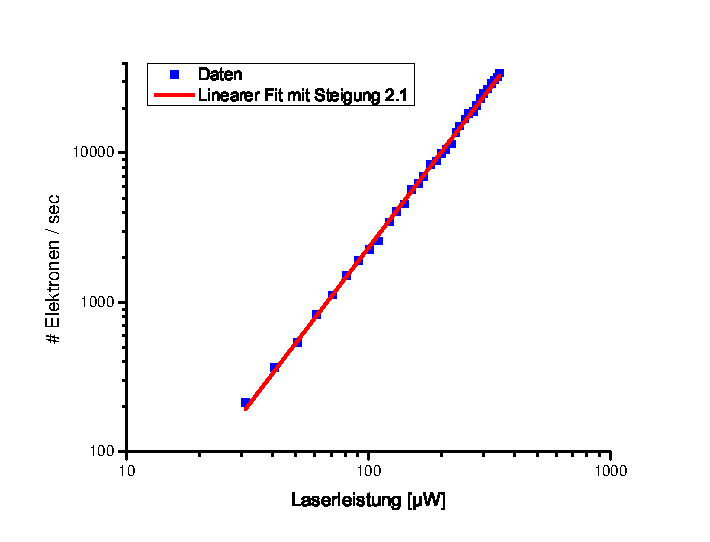
\includegraphics[width=0.49\textwidth]{480e}}
  \hfill
  \subfigure[520nm - Gefittete Steigung ohne die letzten 28 Werte: $2.6\pm0.1$\label{fig:520e}]
  {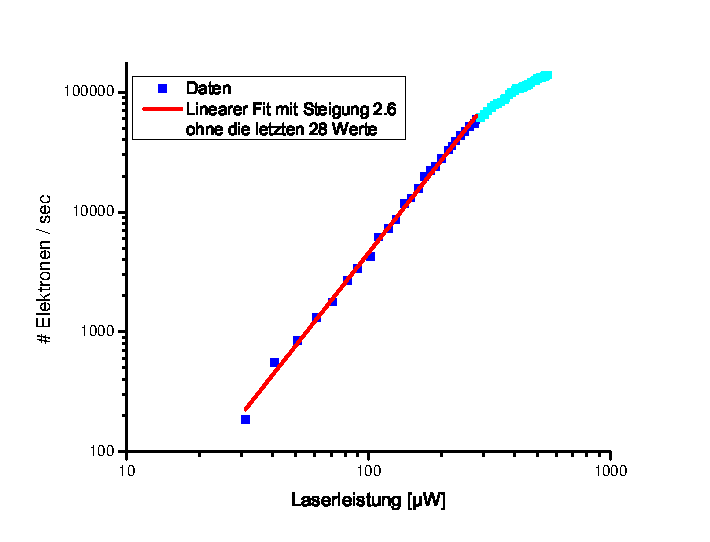
\includegraphics[width=0.49\textwidth]{520e}}
  \hfill
  \subfigure[690nm - Gefittete Steigung: $3.7\pm0.1$\label{fig:690e}]
  {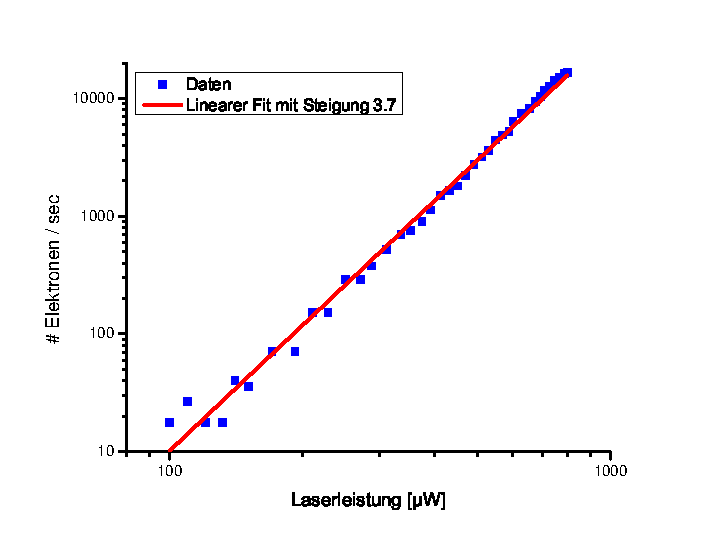
\includegraphics[width=0.49\textwidth]{690e}}
  \caption{Beispielhafte Auftragung des Elektronenstroms gegen die eingestrahlte mittlere Laserleistung zu drei beispielhaften Wellenlängen.}
  \label{fig:e}
\end{figure}


\begin{figure}[h]
	\centering
	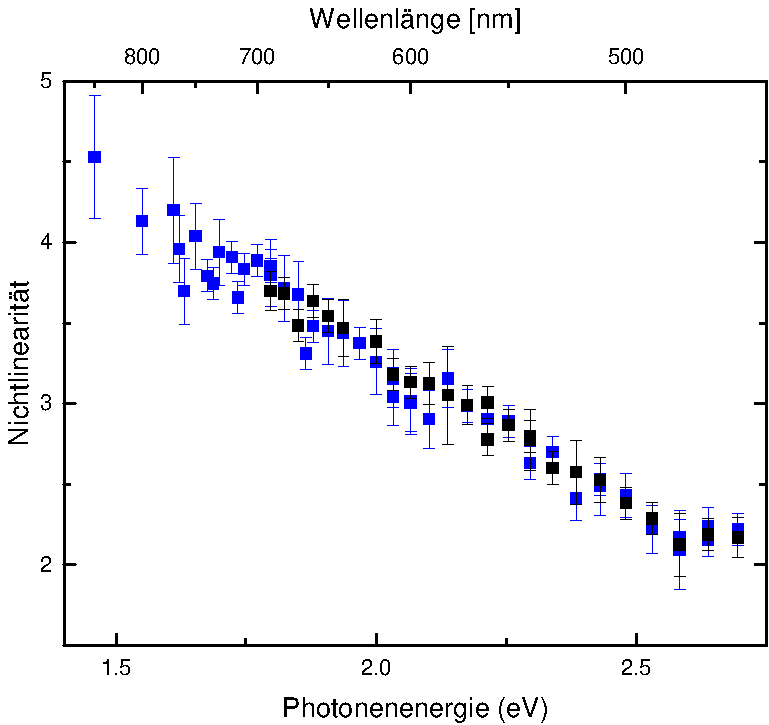
\includegraphics[width=0.8\linewidth]{Vergleich}
	\caption{Vergleich der ersten mit der zweiten Messung der Nichtlinearität in dem doppelt vermessenen Wellenlängenbereich. Zu erkennen ist, dass die beiden Messreihen vergleichbare Ergebnisse lieferten und meist in den Fehlerintervallen der jeweils anderen.}
	\label{fig:ges_messung}
\end{figure}

Plottet man wie in Abb. \ref{fig:ges_messung} zu sehen die Steigung gegen die Wellenlänge, so ergibt sich nicht das einfachste zu erwartende Bild einer Treppenfunktion, was aus Gleichung \ref{eq:nomega} folgen würde.
Stattdessen sind die Daten annähernd linear mit kleinen Plateaus um die ganzzahligen Nichtlinearitäten.
Effekte, welche zu einer ``Linearisierung'' der Stufenfunktion führen können sind thermisches Heizen, niederenergetische Elektronen, das $d$-Band, thermisches Tunneln und unterschiedliche Facetten.
Dies wird in Kapitel \ref{sec:erklaerung_lin} weiter ausgeführt.
Die eingezeichneten Fehler sind eine Kombination der Fehler aus den Fits und einem systematischen Fehler, der mit 0.1 angenommen wurde.

\newpage
In Abb. \ref{fig:ges_messung} sind zwei Messreihen eingetragen.
Diese sind mit gleichen Parametern aufgenommen worden, jedoch wurde bei den in schwarz eingezeichneten Daten vermehrt darauf geachtet, dass die Position des Laserstrahls auf der Spitze korrekt ist.
Zu erkennen ist, dass die Kurven überwiegend in guter Übereinstimmung liegen und die Ausreißer durch Datenpunkte der jeweils anderen Kurve ausgeglichen werden.
Allerdings ist es nicht auszuschließen, dass manche der Messwerte in blau nicht am Apex, sondern an dem nächsten hellen Spot $\SI{20}{\micro\meter}$ von der Spitze entfernt aufgenommen wurden.
Hier wird ein Defekt vermutet, welcher ebenfalls zu einem starken Elektronensignal führt.
Dies führt dazu, dass manche Werte deutliche Abweichungen von der Kurve zeigen.
Es ist vermutlich nicht darin begründet, dass die Messungen sehr streuen, da erneute Messungen an exakt den selben Positionen kaum Abweichungen hatten.\\\\

In Grafik \ref{fig:stufen} sind zusätzlich zu den Messwerten aus Abb. \ref{fig:ges_messung} noch Stufenfunktionen mit unterschiedliche Austrittsarbeiten eingezeichnet.
Deutlich zu erkennen ist, dass die Werte oberhalb der Kurve für die niedrigste in der Literatur angegebene Austrittsarbeit liegt.
Die Daten liegen auch alle unterhalb der Austrittsarbeit des $d$-Bandes.

\begin{figure}[h!]
	\centering
	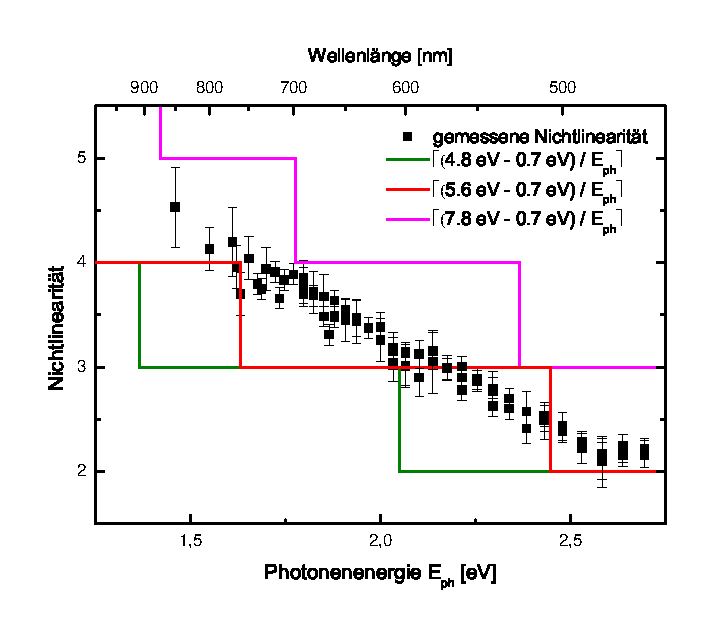
\includegraphics{Stufen}
	\caption{Daten aus Abb. \ref{fig:ges_messung} zusammen mit dem einfachsten denkbaren Modell, welches Stufen vorhersagt. Eingetragen sind in grün mit \SI{4.8}{\eV} Austrittsarbeit ein niedriger Wert der Fermienergie aus \cite{trasatti_operative_1974}, welcher die Daten nach unten hin begrenzen sollte. In rot ist der höchste Wert einer Austrittsarbeit für eine Facette nach \cite{crc} eingezeichnet als Referenz, um zu sehen, ob Elektronen ausschließlich von der Fermikante kommen. Wäre dies der Fall, so müssten die Daten zwischen den beiden Kurven liegen. In pink ist dann die ungefähre Lage des $d$-Bandes eingezeichnet. Klar zu erkennen ist, dass die Messwerte zwischen der grünen und der pinken, jedoch auf beiden Seiten der roten Kurve liegen.}
	\label{fig:stufen}
\end{figure}

\newpage
Weitere Einblicke in die Daten liefert die mittlere Energie, die bei einem Emissionsprozess umgesetzt wird.
Dies wurde in Abb. \ref{fig:ges_energie} für die Nichtlinearitäten aus Diagramm \ref{fig:ges_messung} getan, indem sie mit der Photonenenergie der jeweiligen Wellenlänge multipliziert wurden.
Zu erkennen ist, dass der niedrigste Wert bei $\SI{480}{\nano\meter}$ eine Energie von $\SI{5.49}\electronvolt$ vorliegt, was gut zu den Literaturwerten passt.
Höhere Werte lassen sich zum Beispiel durch kinetische Energie der Elektronen oder die in Kap. \ref{sec:erklaerung_lin} aufgeführten Effekte erklären.
%Dass die Gesamtenergie bei einem Emissionsprozess mit größeren Wellenlängen ansteigt, lässt sich damit erklären, dass bei größeren benötigten Photonenanzahlen die Wahrscheinlichkeit, dass ein weiteres zeitgleich ankommt, größer ist.
Bei höheren Ordnungen $N$ steigt der relative Wirkungsquerschnitt $\sigma_N$ aus Gleichung \ref{eq:wirkungsquerschnitt} von Prozessen mit einer ähnlichen Anzahl an Photonen.
Mit dieser zusätzlichen Energie ist es dann jedoch möglich, nicht nur Elektronen von der Fermi-Kante, sondern auch aus dem $d$-Band zu emittieren.
Da es von diesen jedoch nach Kapitel \ref{sec:zustandsdichte} um eine Größenordnung mehr Elektronen gibt, steigt die Wahrscheinlichkeit einer Emission.\newline\newline



 



\begin{figure}[h!]
\centering
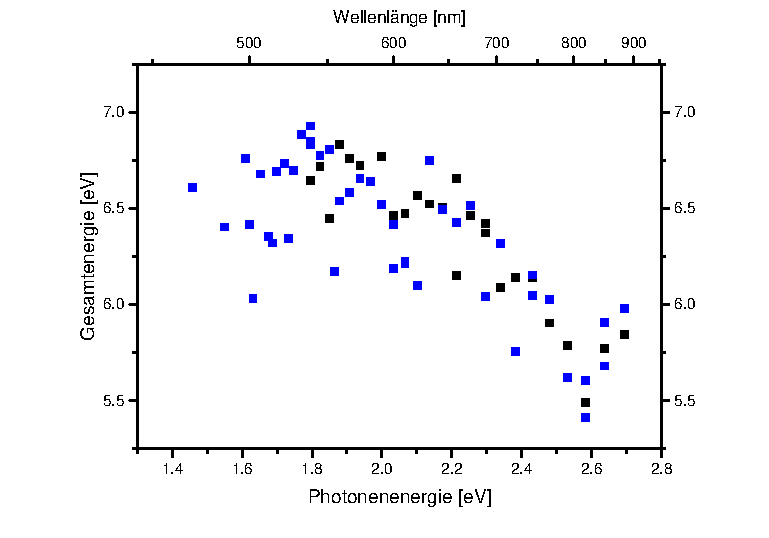
\includegraphics{Gesamtenergie}
\caption{Auftragung der Nichtlinearität aus Abb. \ref{fig:ges_messung} multipliziert mit der jeweiligen Photonenenergie. Zusätzlich eingezeichnet in grün ist eine Gesamtenergie von \SI{5.4}{\eV}, welche über den Austrittsarbeiten aus Tabelle \ref{tab:austrittsarbeit} liegt wenn man den Schottky-Effekt von $\SI{0.7}{\eV}$ mit einberechnet.}
\label{fig:ges_energie}
\end{figure}


\newpage
In Grafik \ref{fig:regenbogen} sind ausgewählte Messreihen zusammen dargestellt.
Erkennbar ist, dass mit steigender Wellenlänge die Geradensteigung zunimmt, der Achsenabschnitt jedoch nicht konstant ist.
Die Farbe der Geraden entspricht in etwa der des Lichtes, bei der die Gerade gefittet wurde.
Erkennbar ist, dass die Achsenabschnitte nicht gleich sind zwischen verschiedenen Messreihen, was zum Beispiel durch eine unterschiedlich starke Fokussierung verschiedener Wellenlängen zu erklären ist.
Die Steigung der einzelnen Kurven nimmt mit steigender Wellenlänge offensichtlich zu.


\begin{figure}[h!]
	\centering
	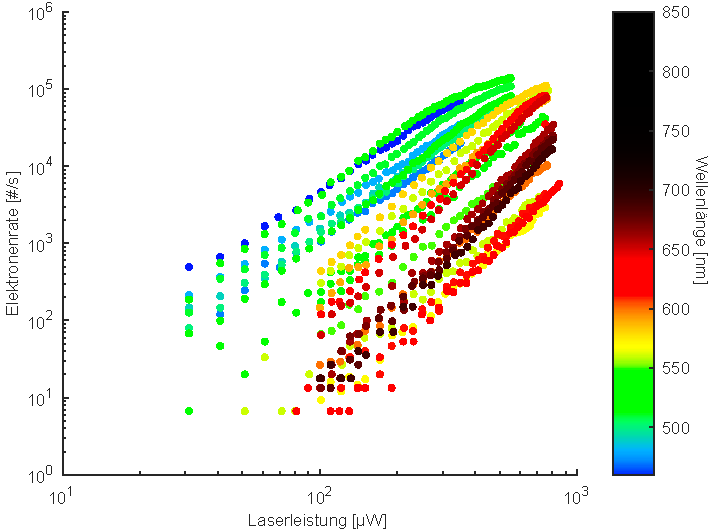
\includegraphics[width=0.7\textwidth]{Faecher_Daten}
	\caption{Ausgewählte Messreihen verschiedener Wellenlängen aufgetragen. Die Farbe der Messpunkte entspricht in etwa der wahrgenommenen Farbe des Lichts.}
	\label{fig:regenbogen}
\end{figure}


% \section{Spannungsscan}
% Der zweite Teil der Messung bestand in einem Spannungsscan.
% Dabei wurde bei konstanter Wellenlänge die Spannung in \SI{20}{\V} Schritten von 500 auf \SI{100}{\V} gesenkt.




\chapter{Diskussion und Ausblick}
In diesem Abschnitt soll auf mögliche Fehlerquellen eingegangen werden, sowie ein Ausblick auf mögliche zukünftige ergänzende Experimente gegeben werden.

\section{Stabilität der Laserintensität}
Die SHG ist sehr sensitiv auf das interne Beampointing, so dass selbst ein relativ geringer Luftzug mit seinen Dichteschwankungen schon deutliche Einbrüche in der Intensität bedeutet.
Dies bedeutet, dass selbst das Vorbeigehen am Laser Einbrüche von bis zu 50\% an Leistung bewirkte.
Die Feedback-Schleife war jedoch nicht darauf ausgelegt, kontinuierlich zu regeln, sondern stellte nur zu Beginn jeder Messung die Intensität ein.
Während die Bilder aufgenommen wurden regelte sie also nicht nach.
Da jedoch nicht viele Personen an dem Lasersystem vorbeigingen und im späteren Verlauf der Messungen darauf geachtet wurde, dass während der Messungen kein Luftzug entstand, sind höchstens einzelne Datenpunkte von einzelnen Wellenlängen betroffen.


\section{Degradation der Spitze}
In Abb. \ref{fig:rem} sind REM-Aufnahmen der verwendeten Spitze vor und nach dem Experiment gezeigt.
Deutlich zu sehen ist, dass nach den Messungen sich Strukturen auf der Spitze befanden.
Diese Hahnenkamm-ähnlichen Auswüchse haben sehr viel kleinere Radien.
Allerdings ist es möglich, dass sie erst entstanden, als die Spitze aus der Vakuumkammer genommen wurde, um sie ins REM einzubauen.
Bild \ref{fig:spitze_vorher2} ist zwar etwas unscharf, jedoch scheint auch da schon der Krümmungsradius des Apexes gegenüber \ref{fig:spitze_vorher} größer zu sein und eine Ausbuchtung nach oben entstanden zu sein.
Dies ist insofern wahrscheinlich, als dass die Spitze vor dem Ausbau nicht besonders viele Elektronen emittiert hat, wie es bei einer hohen Feldüberhöhung zu erwarten gewesen wäre.
Auch lässt sich ein leichter Farbkontrast zwischen der Spitze und dem gewachsenen erkennen, was dafür spricht, dass es sich bei dem angelagerten Material nicht um Gold handelt.
Denkbar wäre es, dass beim Ausbau durch elektrostatische Felder Schmutz angezogen wurde und sich niedergeschlagen hat.

\begin{figure}[h!]
  \centering
  \subfigure[REM-Bild der Spitze vom 12.06.14\label{fig:spitze_vorher}]
  {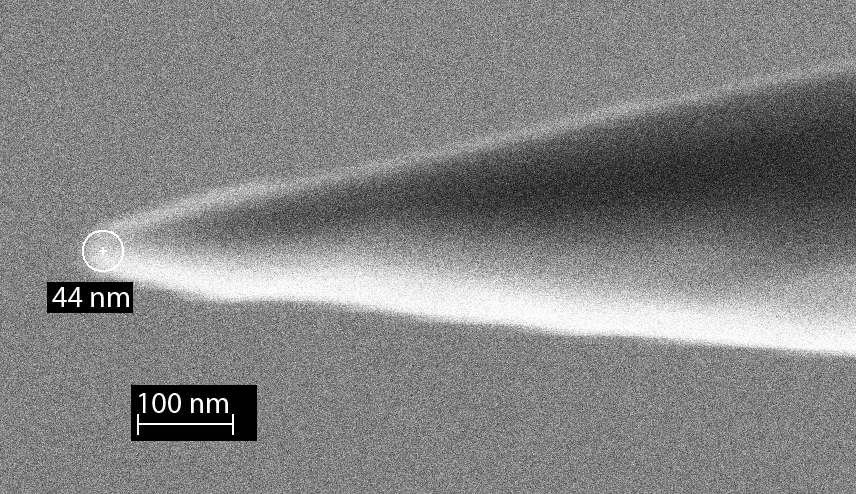
\includegraphics[width=0.49\textwidth]{spitze_vorher}}
  \hfill
  \subfigure[REM-Bild der Spitze vom 23.10.14\label{fig:spitze_vorher2}]
  {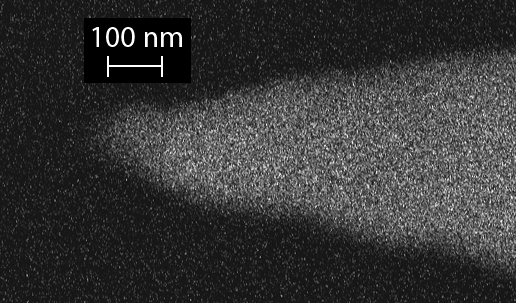
\includegraphics[width=0.49\textwidth]{spitze_vorher2}}
  \hfill
  \subfigure[REM-Bild der Spitze vom 31.05.16\label{fig:spitze_nachher}]
  {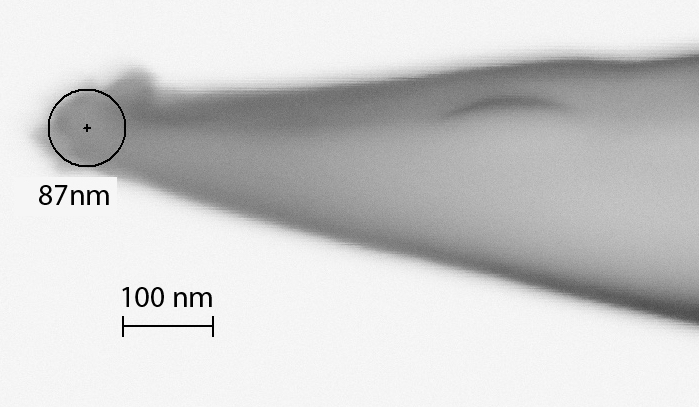
\includegraphics[width=0.49\textwidth]{spitze_nachher}}
  \caption{REM-Bild der Spitze vor und nach den Messungen.}
  \label{fig:rem}
\end{figure}

Als Strahler, der sich ungefähr in der Mitte zwischen Apex und Gitter befand könnten die zwei Körner mit einem Durchmesser von 230 und \SI{270}{\nm} fungiert haben (s. Bild \ref{fig:hotspots}.

\begin{figure}[h]
	\centering
	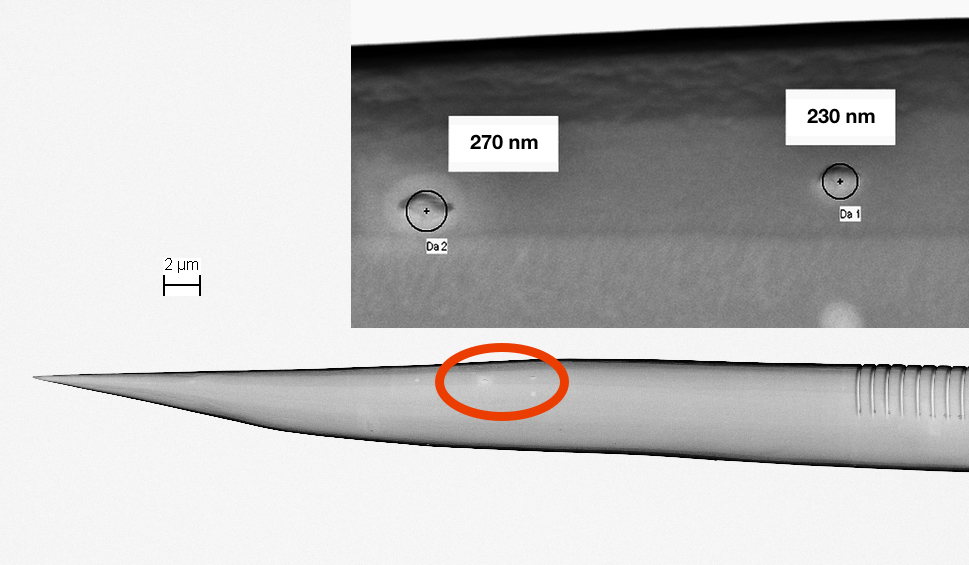
\includegraphics[width=0.8\linewidth]{Hotspots}
	\caption{Körner auf der Spitze, welche sich zwischen Apex und Gitter befanden. Diese wurden teilweise bei einer ersten Messreihe vermutlich beleuchtet.}
	\label{fig:hotspots}
\end{figure}



\section{Effekte zur Linearisierung der Daten}
\label{sec:erklaerung_lin}
Die Daten in Grafik \ref{fig:ges_messung} scheinen zunächst annähernd linear zu sein.
Bei genauerer Betrachtung fällt auf, dass sich Ansätze von Plateaus bei den ganzzahligen Nichtlinearitäten ausmachen lassen.
Fittet man die ermittelten Ordnungen linear, so ergibt sich eine Steigung von $\SI{-2}{\per\eV}$.

Die folgenden Effekte können zu einer Glättung der Stufenfunktion führen:
\begin{itemize}
	\item Durch den Energieeintrag in die Spitze wird diese aufgeheizt. Die Elektronen werden so angeregt und benötigen gegebenenfalls weniger Photonen, als bei Raumtemperatur oder dem absoluten Nullpunkt.
	\item Wie in Kapitel \ref{sec:zustandsdichte} beschrieben, existieren nicht nur Elektronen an der Fermi-Kante. Daher können sowohl Elektronen niedrigerer, als auch (jedoch weniger) höherer Energie ausgelöst werden.
	\item In dem $d$-Band befinden sich um eine Größenordnung mehr Elektronen, als an der Fermikante (s. Kap. \ref{sec:zustandsdichte}). Daher trifft der vorherige Punkt besonders stark für diesen Energiebereich zu.
	\item Durch den Schottky-Effekt (Kap. \ref{sec:schottky}) findet eine Erniedrigung der effektiven Austrittsarbeit statt. Thermisch angeregte Elektronen können somit tunneln (entweder durch Photo-assisted field-emission oder durch einen reinen Tunnelprozess).
	\item Zudem führen die unterschiedlichen Kristall-Facetten mit unterschiedlichen Austrittsarbeiten zu einer Glättung der Kurve. Dies ist der Fall, da sich die unterschiedlichen Steigungen überlagern in den Bereichen, wo die Flächen eine unterschiedliche Ordnung in der Nichtlinearität haben.
\end{itemize}

Dies führt dazu, dass man sowohl energiearme, als auch energiereiche Elektronen detektieren können müsste.
Dies wäre im Rahmen einer zukünftigen Messreihe empfehlenswert zu überprüfen.
Sollte die Hypothese der Überlagerung verschiedener Multiphotonen-Prozesse zutreffen, so kann man bei größeren Wellenlängen keine energetisch schmalbandigen Elektronen zum Beispiel für das Ultrafast Low Energy Electron Defraction (ULEED) Experiment mit dieser Methode bereitstellen.
Dies benötigt sehr schmalbandige Elektronenspektren, damit die Elektronenpulse durch Dispersion nicht zu stark verlängert werden, was die Zeitauflösung verringern würde \cite{gahlmann_2008}.




\appendix

\chapter{Anhang}
\begin{figure}[h]
	\centering
	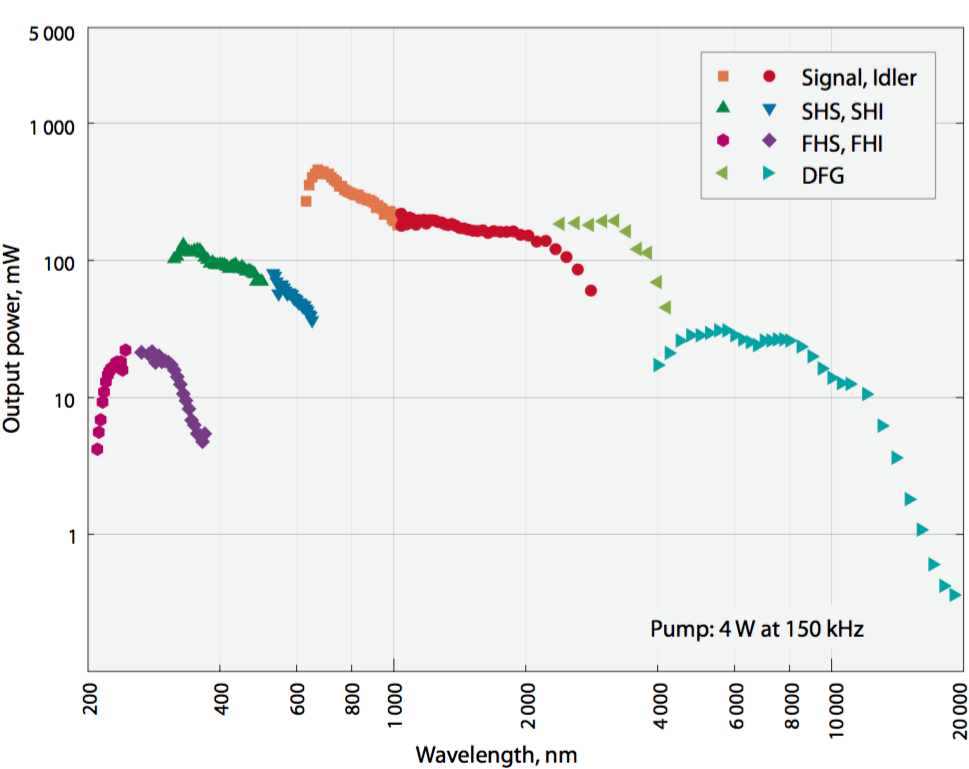
\includegraphics[width=0.7\linewidth]{Orpheus_Tuning_Curve}
	\caption{Ausgangsleistung des Orpheus im gesamten emittierenden Wellenlängenbereich aus dem Datenblatt des Herstellers \protect\footnotemark.}
	\label{fig:orpheus_tuningcurve}
\end{figure}
\footnotetext{Light Conversion Produktkatalog 2013, \url{http://www.lightcon.com/upload/iblock/2db/2db3f7cec5ac57521f58ced3aa1eb9aa.pdf}, Abgerufen 27.06.2016}

\cleardoublepage
%% Bibliographie. Das Argument muss der Name der BIBTeX-Datenbank stehen.
%% Ein Beispiel fuer eine solche Datenbank finden Sie in bthesis_datenbank.bib
\bibliography{bthesis_datenbank}

\chapter*{Danksagung}
Mein Dank geht in erster Linie an Claus Ropers, der mir die Möglichkeit gab, diese äußerst spannende Arbeit durchzuführen und der mir mit fachlichen Anregungen stets zur Seite stand.\\

Ebenfalls möchte ich Dr. Reiner Bormann und Benjamin Schröder für die ausgezeichnete Betreuung danken.
Auch Gerrit Horstmann unterstützte mich stets (nicht nur moralisch mit Eis!).\\

Bei Herrn Prof. Jooß möchte ich mich für die freundliche Bereitschaft bedanken, die Zweitkorrektur zu übernehmen.\\

Der Arbeitsgruppe möchte ich für die ausgesprochen angenehme Athmosphäre sowohl im wissenschaftlichen, als auch im sozialen danken.
Egal mit was für einer Frage ich ankam halfen mir stets alle sehr zuvorkommend.\\

Ebenfalls Dank gebührt Nicolas Wöhrl und Reinhard Remfort vom Podcast \textit{Methodisch Inkorrekt}, da sie mir mit ihren interessanten wissenschaftlichen Themen zahlreiche Stunden im dunklen Labor angenehm gemacht haben.\\\\

Natürlich möchte ich mich nicht zuletzt bei meiner Familie bedanken, dass sie es mir ermöglichen, ein so interessantes Studium zu ermöglichen und mich stets unterstützten.
Eine bessere kann man sich nicht wünschen!


\end{document}
